%% bm.pdf preamble - material merged from previous preamble and current pandoc preamable output
% NOTE: float placement required changes to the source files referenced by bm.tex
% May 28, 2020
%
% Use lualatex to compile - test with MiKTeX 2.9

% uncomment to list all files in log
%\listfiles

\documentclass[12pt]{report}


\usepackage{fontspec}

%\setmainfont[Scale=MatchLowercase]{Lucida Bright}
%\setmonofont{FreeMono}
%\setmonofont{Source Code Pro}
\setmonofont[Scale=MatchLowercase]{Ubuntu Mono}

% short snippets of asian languages
\newfontfamily\myAsian{Noto Serif TC Medium}

\usepackage[headings]{fullpage}

% national use characters 
%\usepackage{inputenc}

% ams mathematical symbols
\usepackage{amsmath,amssymb}

% added to support pandoc highlighting
\usepackage{microtype}

\usepackage{makeidx}

% add index and bibliographies to table of contents
\usepackage[nottoc]{tocbibind}

% postscript courier and times in place of cm fonts
%\usepackage{courier}
%\usepackage{times}

% extended coloring
\usepackage{color}
\usepackage[table,dvipsnames]{xcolor}
\usepackage{colortbl}

% advanced date formating
\usepackage{datetime}

%support pandoc code highlighting
\usepackage{fancyvrb}

% \DefineShortVerb[commandchars=\\\{\}]{\|}
% \DefineVerbatimEnvironment{Highlighting}{Verbatim}{commandchars=\\\{\}}
% % Add ',fontsize=\small' for more characters per line

% tango style colors
% \usepackage{framed}
% \definecolor{shadecolor}{RGB}{255,255,255}
% \newenvironment{Shaded}{\begin{snugshade}}{\end{snugshade}}
% \newcommand{\KeywordTok}[1]{\textcolor[rgb]{0.13,0.29,0.53}{\textbf{{#1}}}}
% \newcommand{\DataTypeTok}[1]{\textcolor[rgb]{0.13,0.29,0.53}{{#1}}}
% \newcommand{\DecValTok}[1]{\textcolor[rgb]{0.00,0.00,0.81}{{#1}}}
% \newcommand{\BaseNTok}[1]{\textcolor[rgb]{0.00,0.00,0.81}{{#1}}}
% \newcommand{\FloatTok}[1]{\textcolor[rgb]{0.00,0.00,0.81}{{#1}}}
% \newcommand{\CharTok}[1]{\textcolor[rgb]{0.31,0.60,0.02}{{#1}}}
% \newcommand{\StringTok}[1]{\textcolor[rgb]{0.31,0.60,0.02}{{#1}}}
% \newcommand{\CommentTok}[1]{\textcolor[rgb]{0.56,0.35,0.01}{\textit{{#1}}}}
% \newcommand{\OtherTok}[1]{\textcolor[rgb]{0.56,0.35,0.01}{{#1}}}
% \newcommand{\AlertTok}[1]{\textcolor[rgb]{0.94,0.16,0.16}{{#1}}}
% \newcommand{\FunctionTok}[1]{\textcolor[rgb]{0.00,0.00,0.00}{{#1}}}
% \newcommand{\RegionMarkerTok}[1]{{#1}}
% \newcommand{\ErrorTok}[1]{\textbf{{#1}}}
% \newcommand{\NormalTok}[1]{{#1}}

% %espresso style colors
% \usepackage{framed}
% \definecolor{shadecolor}{RGB}{42,33,28}
% \newenvironment{Shaded}{\begin{snugshade}}{\end{snugshade}}
% \newcommand{\KeywordTok}[1]{\textcolor[rgb]{0.26,0.66,0.93}{\textbf{{#1}}}}
% \newcommand{\DataTypeTok}[1]{\textcolor[rgb]{0.74,0.68,0.62}{\underline{{#1}}}}
% \newcommand{\DecValTok}[1]{\textcolor[rgb]{0.27,0.67,0.26}{{#1}}}
% \newcommand{\BaseNTok}[1]{\textcolor[rgb]{0.27,0.67,0.26}{{#1}}}
% \newcommand{\FloatTok}[1]{\textcolor[rgb]{0.27,0.67,0.26}{{#1}}}
% \newcommand{\CharTok}[1]{\textcolor[rgb]{0.02,0.61,0.04}{{#1}}}
% \newcommand{\StringTok}[1]{\textcolor[rgb]{0.02,0.61,0.04}{{#1}}}
% \newcommand{\CommentTok}[1]{\textcolor[rgb]{0.00,0.40,1.00}{\textit{{#1}}}}
% \newcommand{\OtherTok}[1]{\textcolor[rgb]{0.74,0.68,0.62}{{#1}}}
% \newcommand{\AlertTok}[1]{\textcolor[rgb]{1.00,1.00,0.00}{{#1}}}
% \newcommand{\FunctionTok}[1]{\textcolor[rgb]{1.00,0.58,0.35}{\textbf{{#1}}}}
% \newcommand{\RegionMarkerTok}[1]{\textcolor[rgb]{0.74,0.68,0.62}{{#1}}}
% \newcommand{\ErrorTok}[1]{\textcolor[rgb]{0.74,0.68,0.62}{\textbf{{#1}}}}
% \newcommand{\NormalTok}[1]{\textcolor[rgb]{0.74,0.68,0.62}{{#1}}}

% %kete style colors
% \newenvironment{Shaded}{}{}
% \newcommand{\KeywordTok}[1]{\textbf{{#1}}}
% \newcommand{\DataTypeTok}[1]{\textcolor[rgb]{0.50,0.00,0.00}{{#1}}}
% \newcommand{\DecValTok}[1]{\textcolor[rgb]{0.00,0.00,1.00}{{#1}}}
% \newcommand{\BaseNTok}[1]{\textcolor[rgb]{0.00,0.00,1.00}{{#1}}}
% \newcommand{\FloatTok}[1]{\textcolor[rgb]{0.50,0.00,0.50}{{#1}}}
% \newcommand{\CharTok}[1]{\textcolor[rgb]{1.00,0.00,1.00}{{#1}}}
% \newcommand{\StringTok}[1]{\textcolor[rgb]{0.87,0.00,0.00}{{#1}}}
% \newcommand{\CommentTok}[1]{\textcolor[rgb]{0.50,0.50,0.50}{\textit{{#1}}}}
% \newcommand{\OtherTok}[1]{{#1}}
% \newcommand{\AlertTok}[1]{\textcolor[rgb]{0.00,1.00,0.00}{\textbf{{#1}}}}
% \newcommand{\FunctionTok}[1]{\textcolor[rgb]{0.00,0.00,0.50}{{#1}}}
% \newcommand{\RegionMarkerTok}[1]{{#1}}
% \newcommand{\ErrorTok}[1]{\textcolor[rgb]{1.00,0.00,0.00}{\textbf{{#1}}}}
% \newcommand{\NormalTok}[1]{{#1}}
% %end pandoc code hacks

% jodliterate colors
\usepackage{color}
\definecolor{shadecolor}{RGB}{248,248,248}
% j control structures 
\definecolor{keywcolor}{rgb}{0.13,0.29,0.53}
% j explicit arguments x y m n u v
\definecolor{datacolor}{rgb}{0.13,0.29,0.53}
% j numbers - all types see j.xml
\definecolor{decvcolor}{rgb}{0.00,0.00,0.81}
\definecolor{basencolor}{rgb}{0.00,0.00,0.81}
\definecolor{floatcolor}{rgb}{0.00,0.00,0.81}
% j local assignments
\definecolor{charcolor}{rgb}{0.31,0.60,0.02}
\definecolor{stringcolor}{rgb}{0.31,0.60,0.02}
\definecolor{commentcolor}{rgb}{0.56,0.35,0.01}
% primitive adverbs and conjunctions
%\definecolor{othercolor}{rgb}{0.56,0.35,0.01}   
\definecolor{othercolor}{RGB}{0,0,255}
% global assignments
\definecolor{alertcolor}{rgb}{0.94,0.16,0.16}
% primitive J verbs and noun names
\definecolor{funccolor}{rgb}{0.00,0.00,0.00}

% custom colors
\definecolor{CodeBackGround}{cmyk}{0.0,0.0,0,0.05}    % light gray
\definecolor{CodeComment}{rgb}{0,0.50,0.00}           % dark green {0,0.45,0.08}
\definecolor{TableStripes}{gray}{0.9}                 % odd/even background in tables

% Colors for the hyperref package
\definecolor{urlcolor}{rgb}{0,.145,.698}
\definecolor{linkcolor}{rgb}{.71,0.21,0.01}
\definecolor{citecolor}{rgb}{.12,.54,.11}

% % Exact colors from NB
\definecolor{incolor}{HTML}{303F9F}
\definecolor{outcolor}{HTML}{D84315}
\definecolor{cellborder}{HTML}{CFCFCF}
\definecolor{cellbackground}{HTML}{F7F7F7}

% % ANSI colors
\definecolor{ansi-black}{HTML}{3E424D}
\definecolor{ansi-black-intense}{HTML}{282C36}
\definecolor{ansi-red}{HTML}{E75C58}
\definecolor{ansi-red-intense}{HTML}{B22B31}
\definecolor{ansi-green}{HTML}{00A250}
\definecolor{ansi-green-intense}{HTML}{007427}
\definecolor{ansi-yellow}{HTML}{DDB62B}
\definecolor{ansi-yellow-intense}{HTML}{B27D12}
\definecolor{ansi-blue}{HTML}{208FFB}
\definecolor{ansi-blue-intense}{HTML}{0065CA}
\definecolor{ansi-magenta}{HTML}{D160C4}
\definecolor{ansi-magenta-intense}{HTML}{A03196}
\definecolor{ansi-cyan}{HTML}{60C6C8}
\definecolor{ansi-cyan-intense}{HTML}{258F8F}
\definecolor{ansi-white}{HTML}{C5C1B4}
\definecolor{ansi-white-intense}{HTML}{A1A6B2}
\definecolor{ansi-default-inverse-fg}{HTML}{FFFFFF}
\definecolor{ansi-default-inverse-bg}{HTML}{000000}
    

% \usepackage{framed}
% \newenvironment{Shaded}{}{}
% \newcommand{\KeywordTok}[1]{\textcolor{keywcolor}{\textbf{{#1}}}}
% \newcommand{\DataTypeTok}[1]{\textcolor{datacolor}{{#1}}}
% %\newcommand{\DecValTok}[1]{\textcolor{decvcolor}{{#1}}}
% \newcommand{\DecValTok}[1]{{#1}} 
% \newcommand{\BaseNTok}[1]{\textcolor{basencolor}{{#1}}}
% \newcommand{\FloatTok}[1]{\textcolor{floatcolor}{{#1}}}
% \newcommand{\CharTok}[1]{\textcolor{charcolor}{\textbf{{#1}}}}
% \newcommand{\StringTok}[1]{\textcolor{stringcolor}{{#1}}}
% \newcommand{\CommentTok}[1]{\textcolor{commentcolor}{\textit{{#1}}}}
% \newcommand{\OtherTok}[1]{\textcolor{othercolor}{{#1}}} 
% \newcommand{\AlertTok}[1]{\textcolor{alertcolor}{\textbf{{#1}}}}
% %\newcommand{\FunctionTok}[1]{\textcolor{funccolor}{{#1}}}
% \newcommand{\FunctionTok}[1]{{#1}}
% \newcommand{\RegionMarkerTok}[1]{{#1}}
% \newcommand{\ErrorTok}[1]{\textbf{{#1}}}
% \newcommand{\NormalTok}[1]{{#1}}

% The default LaTeX title has an obnoxious amount of whitespace. By default,
% titling removes some of it. It also provides customization options.
\usepackage{titling}

% headers and footers
\usepackage{fancyhdr}
%\pagestyle{fancy}
\pagestyle{plain}

\fancyhead{}
\fancyfoot{}

%\fancyhead[LE,RO]{\slshape \rightmark}
%\fancyhead[LO,RE]{\slshape \leftmark}
\fancyfoot[C]{\thepage}
%\headrulewidth 0.4pt
%\footrulewidth 0 pt

%\addtolength{\headheight}{\baselineskip}

%\lfoot{\emph{Analyze the Data not the Drivel}}
%\rfoot{\emph{\today}}

% subfigure handles figures that contain subfigures
%\usepackage{color,graphicx,subfigure,sidecap}
\usepackage{graphicx,sidecap}
\usepackage{subfigure}
\graphicspath{{./inclusions/}}

% floatflt provides for text wrapping around small figures and tables
\usepackage{floatflt}

% tweak caption formats 
\usepackage{caption} 
\usepackage{sidecap}
%\usepackage{subcaption} % not compatible with subfigure

\usepackage{rotating} % flip tables sideways

% complex footnotes
%\usepackage{bigfoot}

% weird logos \XeLaTeX
\usepackage{metalogo}

\newcommand{\HRule}{\rule{\linewidth}{0.5mm}}

\usepackage[breakable]{tcolorbox}

\usepackage{parskip} % Stop auto-indenting (to mimic markdown behaviour)
    
% Basic figure setup, for now with no caption control since it's done
% automatically by Pandoc (which extracts ![](path) syntax from Markdown).
\usepackage{graphicx}

%\DeclareCaptionFormat{nocaption}{}
%\captionsetup{format=nocaption,aboveskip=0pt,belowskip=0pt}

\usepackage[Export]{adjustbox} % Used to constrain images to a maximum size
\adjustboxset{max size={0.9\linewidth}{0.9\paperheight}}
\usepackage{float}

%\floatplacement{figure}{H} % forces figures to be placed at the correct location

\usepackage{xcolor} % Allow colors to be defined
\usepackage{enumerate} % Needed for markdown enumerations to work
\usepackage{geometry} % Used to adjust the document margins

%\usepackage{amsmath} % Equations
%\usepackage{amssymb} % Equations

\usepackage{textcomp} % defines textquotesingle

% Hack from http://tex.stackexchange.com/a/47451/13684:
\AtBeginDocument{%
	\def\PYZsq{\textquotesingle}% Upright quotes in Pygmentized code
}

\usepackage{upquote} % Upright quotes for verbatim code
\usepackage{eurosym} % defines \euro
\usepackage[mathletters]{ucs} % Extended unicode (utf-8) support

%\usepackage{fancyvrb} % verbatim replacement that allows latex

\usepackage{grffile} % extends the file name processing of package graphics 
					 % to support a larger range
					 
\makeatletter % fix for grffile with XeLaTeX
\def\Gread@@xetex#1{%
  \IfFileExists{"\Gin@base".bb}%
  {\Gread@eps{\Gin@base.bb}}%
  {\Gread@@xetex@aux#1}%
}
\makeatother

% The hyperref package gives us a pdf with properly built
% internal navigation ('pdf bookmarks' for the table of contents,
% internal cross-reference links, web links for URLs, etc.)
\usepackage{hyperref}
% The default LaTeX title has an obnoxious amount of whitespace. By default,
% titling removes some of it. It also provides customization options.
\usepackage{titling}
\usepackage{longtable} % longtable support required by pandoc >1.10
\usepackage{booktabs}  % table support for pandoc > 1.12.2
\usepackage[inline]{enumitem} % IRkernel/repr support (it uses the enumerate* environment)
\usepackage[normalem]{ulem} % ulem is needed to support strikethroughs (\sout)
							% normalem makes italics be italics, not underlines
\usepackage{mathrsfs}

% commands and environments needed by pandoc snippets
% extracted from the output of `pandoc -s`
\providecommand{\tightlist}{%
  \setlength{\itemsep}{0pt}\setlength{\parskip}{0pt}}
  
\DefineVerbatimEnvironment{Highlighting}{Verbatim}{commandchars=\\\{\}}
% Add ',fontsize=\small' for more characters per line
\newenvironment{Shaded}{}{}
\newcommand{\KeywordTok}[1]{\textcolor[rgb]{0.00,0.44,0.13}{\textbf{{#1}}}}
\newcommand{\DataTypeTok}[1]{\textcolor[rgb]{0.56,0.13,0.00}{{#1}}}
\newcommand{\DecValTok}[1]{\textcolor[rgb]{0.25,0.63,0.44}{{#1}}}
\newcommand{\BaseNTok}[1]{\textcolor[rgb]{0.25,0.63,0.44}{{#1}}}
\newcommand{\FloatTok}[1]{\textcolor[rgb]{0.25,0.63,0.44}{{#1}}}
\newcommand{\CharTok}[1]{\textcolor[rgb]{0.25,0.44,0.63}{{#1}}}
\newcommand{\StringTok}[1]{\textcolor[rgb]{0.25,0.44,0.63}{{#1}}}
\newcommand{\CommentTok}[1]{\textcolor[rgb]{0.38,0.63,0.69}{\textit{{#1}}}}
\newcommand{\OtherTok}[1]{\textcolor[rgb]{0.00,0.44,0.13}{{#1}}}
\newcommand{\AlertTok}[1]{\textcolor[rgb]{1.00,0.00,0.00}{\textbf{{#1}}}}
\newcommand{\FunctionTok}[1]{\textcolor[rgb]{0.02,0.16,0.49}{{#1}}}
\newcommand{\RegionMarkerTok}[1]{{#1}}
\newcommand{\ErrorTok}[1]{\textcolor[rgb]{1.00,0.00,0.00}{\textbf{{#1}}}}
\newcommand{\NormalTok}[1]{{#1}}

% Additional commands for more recent versions of Pandoc
\newcommand{\ConstantTok}[1]{\textcolor[rgb]{0.53,0.00,0.00}{{#1}}}
\newcommand{\SpecialCharTok}[1]{\textcolor[rgb]{0.25,0.44,0.63}{{#1}}}
\newcommand{\VerbatimStringTok}[1]{\textcolor[rgb]{0.25,0.44,0.63}{{#1}}}
\newcommand{\SpecialStringTok}[1]{\textcolor[rgb]{0.73,0.40,0.53}{{#1}}}
\newcommand{\ImportTok}[1]{{#1}}
\newcommand{\DocumentationTok}[1]{\textcolor[rgb]{0.73,0.13,0.13}{\textit{{#1}}}}
\newcommand{\AnnotationTok}[1]{\textcolor[rgb]{0.38,0.63,0.69}{\textbf{\textit{{#1}}}}}
\newcommand{\CommentVarTok}[1]{\textcolor[rgb]{0.38,0.63,0.69}{\textbf{\textit{{#1}}}}}
\newcommand{\VariableTok}[1]{\textcolor[rgb]{0.10,0.09,0.49}{{#1}}}
\newcommand{\ControlFlowTok}[1]{\textcolor[rgb]{0.00,0.44,0.13}{\textbf{{#1}}}}
\newcommand{\OperatorTok}[1]{\textcolor[rgb]{0.40,0.40,0.40}{{#1}}}
\newcommand{\BuiltInTok}[1]{{#1}}
\newcommand{\ExtensionTok}[1]{{#1}}
\newcommand{\PreprocessorTok}[1]{\textcolor[rgb]{0.74,0.48,0.00}{{#1}}}
\newcommand{\AttributeTok}[1]{\textcolor[rgb]{0.49,0.56,0.16}{{#1}}}
\newcommand{\InformationTok}[1]{\textcolor[rgb]{0.38,0.63,0.69}{\textbf{\textit{{#1}}}}}
\newcommand{\WarningTok}[1]{\textcolor[rgb]{0.38,0.63,0.69}{\textbf{\textit{{#1}}}}}

% Define a nice break command that doesn't care if a line doesn't already exist.
\def\br{\hspace*{\fill} \\* }
% Math Jax compatibility definitions
\def\gt{>}
\def\lt{<}
\let\Oldtex\TeX
\let\Oldlatex\LaTeX
\renewcommand{\TeX}{\textrm{\Oldtex}}
\renewcommand{\LaTeX}{\textrm{\Oldlatex}}
 
% Pygments definitions
\makeatletter
\def\PY@reset{\let\PY@it=\relax \let\PY@bf=\relax%
    \let\PY@ul=\relax \let\PY@tc=\relax%
    \let\PY@bc=\relax \let\PY@ff=\relax}
\def\PY@tok#1{\csname PY@tok@#1\endcsname}
\def\PY@toks#1+{\ifx\relax#1\empty\else%
    \PY@tok{#1}\expandafter\PY@toks\fi}
\def\PY@do#1{\PY@bc{\PY@tc{\PY@ul{%
    \PY@it{\PY@bf{\PY@ff{#1}}}}}}}
\def\PY#1#2{\PY@reset\PY@toks#1+\relax+\PY@do{#2}}

\expandafter\def\csname PY@tok@w\endcsname{\def\PY@tc##1{\textcolor[rgb]{0.73,0.73,0.73}{##1}}}
\expandafter\def\csname PY@tok@c\endcsname{\let\PY@it=\textit\def\PY@tc##1{\textcolor[rgb]{0.25,0.50,0.50}{##1}}}
\expandafter\def\csname PY@tok@cp\endcsname{\def\PY@tc##1{\textcolor[rgb]{0.74,0.48,0.00}{##1}}}
\expandafter\def\csname PY@tok@k\endcsname{\let\PY@bf=\textbf\def\PY@tc##1{\textcolor[rgb]{0.00,0.50,0.00}{##1}}}
\expandafter\def\csname PY@tok@kp\endcsname{\def\PY@tc##1{\textcolor[rgb]{0.00,0.50,0.00}{##1}}}
\expandafter\def\csname PY@tok@kt\endcsname{\def\PY@tc##1{\textcolor[rgb]{0.69,0.00,0.25}{##1}}}
\expandafter\def\csname PY@tok@o\endcsname{\def\PY@tc##1{\textcolor[rgb]{0.40,0.40,0.40}{##1}}}
\expandafter\def\csname PY@tok@ow\endcsname{\let\PY@bf=\textbf\def\PY@tc##1{\textcolor[rgb]{0.67,0.13,1.00}{##1}}}
\expandafter\def\csname PY@tok@nb\endcsname{\def\PY@tc##1{\textcolor[rgb]{0.00,0.50,0.00}{##1}}}
\expandafter\def\csname PY@tok@nf\endcsname{\def\PY@tc##1{\textcolor[rgb]{0.00,0.00,1.00}{##1}}}
\expandafter\def\csname PY@tok@nc\endcsname{\let\PY@bf=\textbf\def\PY@tc##1{\textcolor[rgb]{0.00,0.00,1.00}{##1}}}
\expandafter\def\csname PY@tok@nn\endcsname{\let\PY@bf=\textbf\def\PY@tc##1{\textcolor[rgb]{0.00,0.00,1.00}{##1}}}
\expandafter\def\csname PY@tok@ne\endcsname{\let\PY@bf=\textbf\def\PY@tc##1{\textcolor[rgb]{0.82,0.25,0.23}{##1}}}
\expandafter\def\csname PY@tok@nv\endcsname{\def\PY@tc##1{\textcolor[rgb]{0.10,0.09,0.49}{##1}}}
\expandafter\def\csname PY@tok@no\endcsname{\def\PY@tc##1{\textcolor[rgb]{0.53,0.00,0.00}{##1}}}
\expandafter\def\csname PY@tok@nl\endcsname{\def\PY@tc##1{\textcolor[rgb]{0.63,0.63,0.00}{##1}}}
\expandafter\def\csname PY@tok@ni\endcsname{\let\PY@bf=\textbf\def\PY@tc##1{\textcolor[rgb]{0.60,0.60,0.60}{##1}}}
\expandafter\def\csname PY@tok@na\endcsname{\def\PY@tc##1{\textcolor[rgb]{0.49,0.56,0.16}{##1}}}
\expandafter\def\csname PY@tok@nt\endcsname{\let\PY@bf=\textbf\def\PY@tc##1{\textcolor[rgb]{0.00,0.50,0.00}{##1}}}
\expandafter\def\csname PY@tok@nd\endcsname{\def\PY@tc##1{\textcolor[rgb]{0.67,0.13,1.00}{##1}}}
\expandafter\def\csname PY@tok@s\endcsname{\def\PY@tc##1{\textcolor[rgb]{0.73,0.13,0.13}{##1}}}
\expandafter\def\csname PY@tok@sd\endcsname{\let\PY@it=\textit\def\PY@tc##1{\textcolor[rgb]{0.73,0.13,0.13}{##1}}}
\expandafter\def\csname PY@tok@si\endcsname{\let\PY@bf=\textbf\def\PY@tc##1{\textcolor[rgb]{0.73,0.40,0.53}{##1}}}
\expandafter\def\csname PY@tok@se\endcsname{\let\PY@bf=\textbf\def\PY@tc##1{\textcolor[rgb]{0.73,0.40,0.13}{##1}}}
\expandafter\def\csname PY@tok@sr\endcsname{\def\PY@tc##1{\textcolor[rgb]{0.73,0.40,0.53}{##1}}}
\expandafter\def\csname PY@tok@ss\endcsname{\def\PY@tc##1{\textcolor[rgb]{0.10,0.09,0.49}{##1}}}
\expandafter\def\csname PY@tok@sx\endcsname{\def\PY@tc##1{\textcolor[rgb]{0.00,0.50,0.00}{##1}}}
\expandafter\def\csname PY@tok@m\endcsname{\def\PY@tc##1{\textcolor[rgb]{0.40,0.40,0.40}{##1}}}
\expandafter\def\csname PY@tok@gh\endcsname{\let\PY@bf=\textbf\def\PY@tc##1{\textcolor[rgb]{0.00,0.00,0.50}{##1}}}
\expandafter\def\csname PY@tok@gu\endcsname{\let\PY@bf=\textbf\def\PY@tc##1{\textcolor[rgb]{0.50,0.00,0.50}{##1}}}
\expandafter\def\csname PY@tok@gd\endcsname{\def\PY@tc##1{\textcolor[rgb]{0.63,0.00,0.00}{##1}}}
\expandafter\def\csname PY@tok@gi\endcsname{\def\PY@tc##1{\textcolor[rgb]{0.00,0.63,0.00}{##1}}}
\expandafter\def\csname PY@tok@gr\endcsname{\def\PY@tc##1{\textcolor[rgb]{1.00,0.00,0.00}{##1}}}
\expandafter\def\csname PY@tok@ge\endcsname{\let\PY@it=\textit}
\expandafter\def\csname PY@tok@gs\endcsname{\let\PY@bf=\textbf}
\expandafter\def\csname PY@tok@gp\endcsname{\let\PY@bf=\textbf\def\PY@tc##1{\textcolor[rgb]{0.00,0.00,0.50}{##1}}}
\expandafter\def\csname PY@tok@go\endcsname{\def\PY@tc##1{\textcolor[rgb]{0.53,0.53,0.53}{##1}}}
\expandafter\def\csname PY@tok@gt\endcsname{\def\PY@tc##1{\textcolor[rgb]{0.00,0.27,0.87}{##1}}}
\expandafter\def\csname PY@tok@err\endcsname{\def\PY@bc##1{\setlength{\fboxsep}{0pt}\fcolorbox[rgb]{1.00,0.00,0.00}{1,1,1}{\strut ##1}}}
\expandafter\def\csname PY@tok@kc\endcsname{\let\PY@bf=\textbf\def\PY@tc##1{\textcolor[rgb]{0.00,0.50,0.00}{##1}}}
\expandafter\def\csname PY@tok@kd\endcsname{\let\PY@bf=\textbf\def\PY@tc##1{\textcolor[rgb]{0.00,0.50,0.00}{##1}}}
\expandafter\def\csname PY@tok@kn\endcsname{\let\PY@bf=\textbf\def\PY@tc##1{\textcolor[rgb]{0.00,0.50,0.00}{##1}}}
\expandafter\def\csname PY@tok@kr\endcsname{\let\PY@bf=\textbf\def\PY@tc##1{\textcolor[rgb]{0.00,0.50,0.00}{##1}}}
\expandafter\def\csname PY@tok@bp\endcsname{\def\PY@tc##1{\textcolor[rgb]{0.00,0.50,0.00}{##1}}}
\expandafter\def\csname PY@tok@fm\endcsname{\def\PY@tc##1{\textcolor[rgb]{0.00,0.00,1.00}{##1}}}
\expandafter\def\csname PY@tok@vc\endcsname{\def\PY@tc##1{\textcolor[rgb]{0.10,0.09,0.49}{##1}}}
\expandafter\def\csname PY@tok@vg\endcsname{\def\PY@tc##1{\textcolor[rgb]{0.10,0.09,0.49}{##1}}}
\expandafter\def\csname PY@tok@vi\endcsname{\def\PY@tc##1{\textcolor[rgb]{0.10,0.09,0.49}{##1}}}
\expandafter\def\csname PY@tok@vm\endcsname{\def\PY@tc##1{\textcolor[rgb]{0.10,0.09,0.49}{##1}}}
\expandafter\def\csname PY@tok@sa\endcsname{\def\PY@tc##1{\textcolor[rgb]{0.73,0.13,0.13}{##1}}}
\expandafter\def\csname PY@tok@sb\endcsname{\def\PY@tc##1{\textcolor[rgb]{0.73,0.13,0.13}{##1}}}
\expandafter\def\csname PY@tok@sc\endcsname{\def\PY@tc##1{\textcolor[rgb]{0.73,0.13,0.13}{##1}}}
\expandafter\def\csname PY@tok@dl\endcsname{\def\PY@tc##1{\textcolor[rgb]{0.73,0.13,0.13}{##1}}}
\expandafter\def\csname PY@tok@s2\endcsname{\def\PY@tc##1{\textcolor[rgb]{0.73,0.13,0.13}{##1}}}
\expandafter\def\csname PY@tok@sh\endcsname{\def\PY@tc##1{\textcolor[rgb]{0.73,0.13,0.13}{##1}}}
\expandafter\def\csname PY@tok@s1\endcsname{\def\PY@tc##1{\textcolor[rgb]{0.73,0.13,0.13}{##1}}}
\expandafter\def\csname PY@tok@mb\endcsname{\def\PY@tc##1{\textcolor[rgb]{0.40,0.40,0.40}{##1}}}
\expandafter\def\csname PY@tok@mf\endcsname{\def\PY@tc##1{\textcolor[rgb]{0.40,0.40,0.40}{##1}}}
\expandafter\def\csname PY@tok@mh\endcsname{\def\PY@tc##1{\textcolor[rgb]{0.40,0.40,0.40}{##1}}}
\expandafter\def\csname PY@tok@mi\endcsname{\def\PY@tc##1{\textcolor[rgb]{0.40,0.40,0.40}{##1}}}
\expandafter\def\csname PY@tok@il\endcsname{\def\PY@tc##1{\textcolor[rgb]{0.40,0.40,0.40}{##1}}}
\expandafter\def\csname PY@tok@mo\endcsname{\def\PY@tc##1{\textcolor[rgb]{0.40,0.40,0.40}{##1}}}
\expandafter\def\csname PY@tok@ch\endcsname{\let\PY@it=\textit\def\PY@tc##1{\textcolor[rgb]{0.25,0.50,0.50}{##1}}}
\expandafter\def\csname PY@tok@cm\endcsname{\let\PY@it=\textit\def\PY@tc##1{\textcolor[rgb]{0.25,0.50,0.50}{##1}}}
\expandafter\def\csname PY@tok@cpf\endcsname{\let\PY@it=\textit\def\PY@tc##1{\textcolor[rgb]{0.25,0.50,0.50}{##1}}}
\expandafter\def\csname PY@tok@c1\endcsname{\let\PY@it=\textit\def\PY@tc##1{\textcolor[rgb]{0.25,0.50,0.50}{##1}}}
\expandafter\def\csname PY@tok@cs\endcsname{\let\PY@it=\textit\def\PY@tc##1{\textcolor[rgb]{0.25,0.50,0.50}{##1}}}

\def\PYZbs{\char`\\}
\def\PYZus{\char`\_}
\def\PYZob{\char`\{}
\def\PYZcb{\char`\}}
\def\PYZca{\char`\^}
\def\PYZam{\char`\&}
\def\PYZlt{\char`\<}
\def\PYZgt{\char`\>}
\def\PYZsh{\char`\#}
\def\PYZpc{\char`\%}
\def\PYZdl{\char`\$}
\def\PYZhy{\char`\-}
\def\PYZsq{\char`\'}
\def\PYZdq{\char`\"}
\def\PYZti{\char`\~}
% for compatibility with earlier versions
\def\PYZat{@}
\def\PYZlb{[}
\def\PYZrb{]}
\makeatother

% For linebreaks inside Verbatim environment from package fancyvrb. 
\makeatletter
	\newbox\Wrappedcontinuationbox 
	\newbox\Wrappedvisiblespacebox 
	\newcommand*\Wrappedvisiblespace {\textcolor{red}{\textvisiblespace}} 
	\newcommand*\Wrappedcontinuationsymbol {\textcolor{red}{\llap{\tiny$\m@th\hookrightarrow$}}} 
	\newcommand*\Wrappedcontinuationindent {3ex } 
	\newcommand*\Wrappedafterbreak {\kern\Wrappedcontinuationindent\copy\Wrappedcontinuationbox} 
	% Take advantage of the already applied Pygments mark-up to insert 
	% potential linebreaks for TeX processing. 
	%        {, <, #, %, $, ' and ": go to next line. 
	%        _, }, ^, &, >, - and ~: stay at end of broken line. 
	% Use of \textquotesingle for straight quote. 
	\newcommand*\Wrappedbreaksatspecials {% 
		\def\PYGZus{\discretionary{\char`\_}{\Wrappedafterbreak}{\char`\_}}% 
		\def\PYGZob{\discretionary{}{\Wrappedafterbreak\char`\{}{\char`\{}}% 
		\def\PYGZcb{\discretionary{\char`\}}{\Wrappedafterbreak}{\char`\}}}% 
		\def\PYGZca{\discretionary{\char`\^}{\Wrappedafterbreak}{\char`\^}}% 
		\def\PYGZam{\discretionary{\char`\&}{\Wrappedafterbreak}{\char`\&}}% 
		\def\PYGZlt{\discretionary{}{\Wrappedafterbreak\char`\<}{\char`\<}}% 
		\def\PYGZgt{\discretionary{\char`\>}{\Wrappedafterbreak}{\char`\>}}% 
		\def\PYGZsh{\discretionary{}{\Wrappedafterbreak\char`\#}{\char`\#}}% 
		\def\PYGZpc{\discretionary{}{\Wrappedafterbreak\char`\%}{\char`\%}}% 
		\def\PYGZdl{\discretionary{}{\Wrappedafterbreak\char`\$}{\char`\$}}% 
		\def\PYGZhy{\discretionary{\char`\-}{\Wrappedafterbreak}{\char`\-}}% 
		\def\PYGZsq{\discretionary{}{\Wrappedafterbreak\textquotesingle}{\textquotesingle}}% 
		\def\PYGZdq{\discretionary{}{\Wrappedafterbreak\char`\"}{\char`\"}}% 
		\def\PYGZti{\discretionary{\char`\~}{\Wrappedafterbreak}{\char`\~}}% 
	} 
	% Some characters . , ; ? ! / are not pygmentized. 
	% This macro makes them "active" and they will insert potential linebreaks 
	\newcommand*\Wrappedbreaksatpunct {% 
		\lccode`\~`\.\lowercase{\def~}{\discretionary{\hbox{\char`\.}}{\Wrappedafterbreak}{\hbox{\char`\.}}}% 
		\lccode`\~`\,\lowercase{\def~}{\discretionary{\hbox{\char`\,}}{\Wrappedafterbreak}{\hbox{\char`\,}}}% 
		\lccode`\~`\;\lowercase{\def~}{\discretionary{\hbox{\char`\;}}{\Wrappedafterbreak}{\hbox{\char`\;}}}% 
		\lccode`\~`\:\lowercase{\def~}{\discretionary{\hbox{\char`\:}}{\Wrappedafterbreak}{\hbox{\char`\:}}}% 
		\lccode`\~`\?\lowercase{\def~}{\discretionary{\hbox{\char`\?}}{\Wrappedafterbreak}{\hbox{\char`\?}}}% 
		\lccode`\~`\!\lowercase{\def~}{\discretionary{\hbox{\char`\!}}{\Wrappedafterbreak}{\hbox{\char`\!}}}% 
		\lccode`\~`\/\lowercase{\def~}{\discretionary{\hbox{\char`\/}}{\Wrappedafterbreak}{\hbox{\char`\/}}}% 
		\catcode`\.\active
		\catcode`\,\active 
		\catcode`\;\active
		\catcode`\:\active
		\catcode`\?\active
		\catcode`\!\active
		\catcode`\/\active 
		\lccode`\~`\~ 	
	}
\makeatother

\let\OriginalVerbatim=\Verbatim
\makeatletter
\renewcommand{\Verbatim}[1][1]{%
	%\parskip\z@skip
	\sbox\Wrappedcontinuationbox {\Wrappedcontinuationsymbol}%
	\sbox\Wrappedvisiblespacebox {\FV@SetupFont\Wrappedvisiblespace}%
	\def\FancyVerbFormatLine ##1{\hsize\linewidth
		\vtop{\raggedright\hyphenpenalty\z@\exhyphenpenalty\z@
			\doublehyphendemerits\z@\finalhyphendemerits\z@
			\strut ##1\strut}%
	}%
	% If the linebreak is at a space, the latter will be displayed as visible
	% space at end of first line, and a continuation symbol starts next line.
	% Stretch/shrink are however usually zero for typewriter font.
	\def\FV@Space {%
		\nobreak\hskip\z@ plus\fontdimen3\font minus\fontdimen4\font
		\discretionary{\copy\Wrappedvisiblespacebox}{\Wrappedafterbreak}
		{\kern\fontdimen2\font}%
	}%
	
	% Allow breaks at special characters using \PYG... macros.
	\Wrappedbreaksatspecials
	% Breaks at punctuation characters . , ; ? ! and / need catcode=\active 	
	\OriginalVerbatim[#1,codes*=\Wrappedbreaksatpunct]%
}
\makeatother


% prompt
\makeatletter
\newcommand{\boxspacing}{\kern\kvtcb@left@rule\kern\kvtcb@boxsep}
\makeatother
\newcommand{\prompt}[4]{
	\ttfamily\llap{{\color{#2}[#3]:\hspace{3pt}#4}}\vspace{-\baselineskip}
}
    

% Prevent overflowing lines due to hard-to-break entities
\sloppy 

% Setup hyperref package
\hypersetup{
  breaklinks=true,  % so long urls are correctly broken across lines
  colorlinks=true,
  urlcolor=urlcolor,
  linkcolor=linkcolor,
  citecolor=citecolor,
  pdfauthor={John D. Baker},
  pdftitle={Analyze the Data not the Drivel},
  pdfsubject={Blog},
  pdfcreator={MikTeX+LaTeXe},
  pdfkeywords={blog,wordpress},
  }
  
% Slightly bigger margins than the latex defaults
% \geometry{verbose,tmargin=1in,bmargin=1in,lmargin=1in,rmargin=1in}  

%\usepackage{wrapfig}

% source code listings
\usepackage{listings}

\lstdefinelanguage{bat}
{morekeywords={echo,title,pushd,popd,setlocal,endlocal,off,if,not,exist,set,goto,pause},
sensitive=True,
morecomment=[l]{rem}
}

\lstdefinelanguage{jdoc}
{
morekeywords={},
otherkeywords={assert.,break.,continue.,for.,do.,if.,else.,elseif.,return.,select.,end.
,while.,whilst.,throw.,catch.,catchd.,catcht.,try.,case.,fcase.},
sensitive=True,
morecomment=[l]{NB.},
morestring=[b]',
morestring=[d]',
}

% latex size ordering - can never remember it
% \tiny
% \scriptsize
% \footnotesize
% \small
% \normalsize
% \large
% \Large
% \LARGE
% \huge
% \Huge
 
% listings package settings  
\lstset{%
  language=jdoc,                                % j document settings
  basicstyle=\ttfamily\footnotesize,            
  keywordstyle=\bfseries\color{keywcolor}\footnotesize,
  identifierstyle=\color{black},
  commentstyle=\slshape\color{CodeComment},     % colored slanted comments
  stringstyle=\color{red}\ttfamily,
  showstringspaces=false,                       
  %backgroundcolor=\color{CodeBackGround},       
  frame=single,                                
  framesep=1pt,                                 
  framerule=0.8pt,                             
  rulecolor=\color{CodeBackGround},   
  showspaces=false,
  %columns=fullflexible,
  %numbers=left,
  %numberstyle=\footnotesize,
  %numbersep=9pt,
  tabsize=2,
  showtabs=false,
  captionpos=b
  breaklines=true,                              
  breakindent=5pt                              
}

\lstdefinelanguage{JavaScript}{
  keywords={typeof, new, true, false, catch, function, return, null, catch, switch, var, if, in, while, do, else, case, break},
  ndkeywords={class, export, boolean, throw, implements, import, this},
  ndkeywordstyle=\color{darkgray}\bfseries,
  sensitive=false,
  comment=[l]{//},
  morecomment=[s]{/*}{*/},
  morestring=[b]',
  morestring=[b]"
}

% C# settings
\lstdefinestyle{sharpc}{
language=[Sharp]C,
basicstyle=\ttfamily\scriptsize, 
keywordstyle=\bfseries\color{keywcolor}\scriptsize,
framerule=0pt
}

% for source code listing longer than two use smaller font
\lstdefinestyle{smallersource}{
basicstyle=\ttfamily\scriptsize, 
keywordstyle=\bfseries\color{keywcolor}\scriptsize,
framerule=0pt
}

\lstdefinestyle{resetdefaults}{
language=jdoc,
basicstyle=\ttfamily\footnotesize,  
keywordstyle=\bfseries\color{keywcolor}\footnotesize,                                                               
framerule=0.8pt 
}

% APL UTF8 code points listed for lstlisting processing
\makeatletter
\lst@InputCatcodes
\def\lst@DefEC{%
 \lst@CCECUse \lst@ProcessLetter
  ^^80^^81^^82^^83^^84^^85^^86^^87^^88^^89^^8a^^8b^^8c^^8d^^8e^^8f%
  ^^90^^91^^92^^93^^94^^95^^96^^97^^98^^99^^9a^^9b^^9c^^9d^^9e^^9f%
  ^^a0^^a1^^a2^^a3^^a4^^a5^^a6^^a7^^a8^^a9^^aa^^ab^^ac^^ad^^ae^^af%
  ^^b0^^b1^^b2^^b3^^b4^^b5^^b6^^b7^^b8^^b9^^ba^^bb^^bc^^bd^^be^^bf%
  ^^c0^^c1^^c2^^c3^^c4^^c5^^c6^^c7^^c8^^c9^^ca^^cb^^cc^^cd^^ce^^cf%
  ^^d0^^d1^^d2^^d3^^d4^^d5^^d6^^d7^^d8^^d9^^da^^db^^dc^^dd^^de^^df%
  ^^e0^^e1^^e2^^e3^^e4^^e5^^e6^^e7^^e8^^e9^^ea^^eb^^ec^^ed^^ee^^ef%
  ^^f0^^f1^^f2^^f3^^f4^^f5^^f6^^f7^^f8^^f9^^fa^^fb^^fc^^fd^^fe^^ff%
  ^^^^20ac^^^^0153^^^^0152%
  ^^^^20a7^^^^2190^^^^2191^^^^2192^^^^2193^^^^2206^^^^2207^^^^220a%
  ^^^^2218^^^^2228^^^^2229^^^^222a^^^^2235^^^^223c^^^^2260^^^^2261%
  ^^^^2262^^^^2264^^^^2265^^^^2282^^^^2283^^^^2296^^^^22a2^^^^22a3%
  ^^^^22a4^^^^22a5^^^^22c4^^^^2308^^^^230a^^^^2336^^^^2337^^^^2339%
  ^^^^233b^^^^233d^^^^233f^^^^2340^^^^2342^^^^2347^^^^2348^^^^2349%
  ^^^^234b^^^^234e^^^^2350^^^^2352^^^^2355^^^^2357^^^^2359^^^^235d%
  ^^^^235e^^^^235f^^^^2361^^^^2362^^^^2363^^^^2364^^^^2365^^^^2368%
  ^^^^236a^^^^236b^^^^236c^^^^2371^^^^2372^^^^2373^^^^2374^^^^2375%
  ^^^^2377^^^^2378^^^^237a^^^^2395^^^^25af^^^^25ca^^^^25cb%  
  ^^00}
\lst@RestoreCatcodes
\makeatother

% custom lengths used within minipages
\newcommand{\minindent}{17pt}

\makeindex

\begin{document}

\subsection*{\href{https://bakerjd99.wordpress.com/2013/08/24/yellowstone-and-me/}{Yellowstone and Me}}
\addcontentsline{toc}{subsection}{Yellowstone and Me}


\noindent\emph{Posted: 24 Aug 2013 06:32:35}
\vspace{6pt}


%{[}caption id=``attachment\_4201'' align=``alignright''  width=``213''{]}

%\href{http://conceptcontrol.smugmug.com/Trips/USA-and-Canada/North-Western/i-cJMHzj5/A}{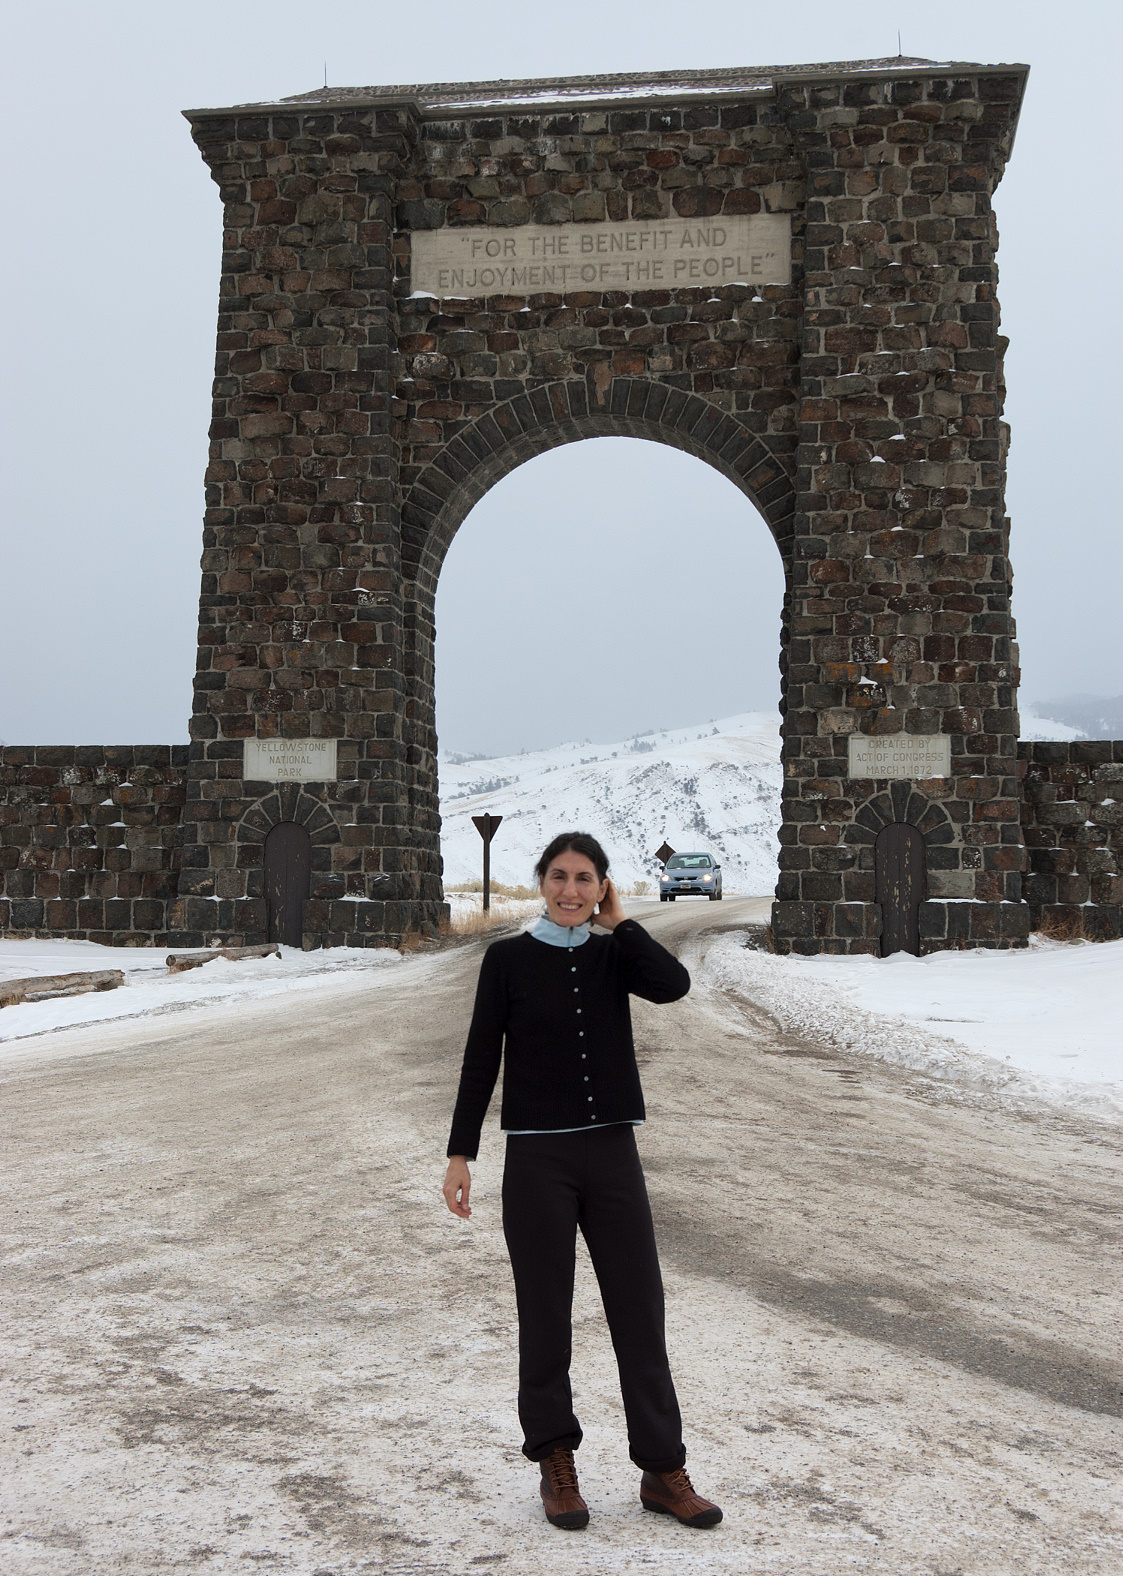
\includegraphics{mali-yellowstone-roosevelt-gate-winter.jpg}}
%My wife in front of the Roosevelt Gate that marks the northern entrance
%to Yellowstone. The road to Mammoth Hot Springs and the Lamar valley are
%open during the winter. Most of the park is snowed under.
%{[}/caption{]}

%\captionsetup[floatingfigure]{labelformat=empty}
%\begin{floatingfigure}[r]{0.35\textwidth}
%\centering
%\href{http://conceptcontrol.smugmug.com/Trips/USA-and-Canada/North-Western/i-cJMHzj5/A}{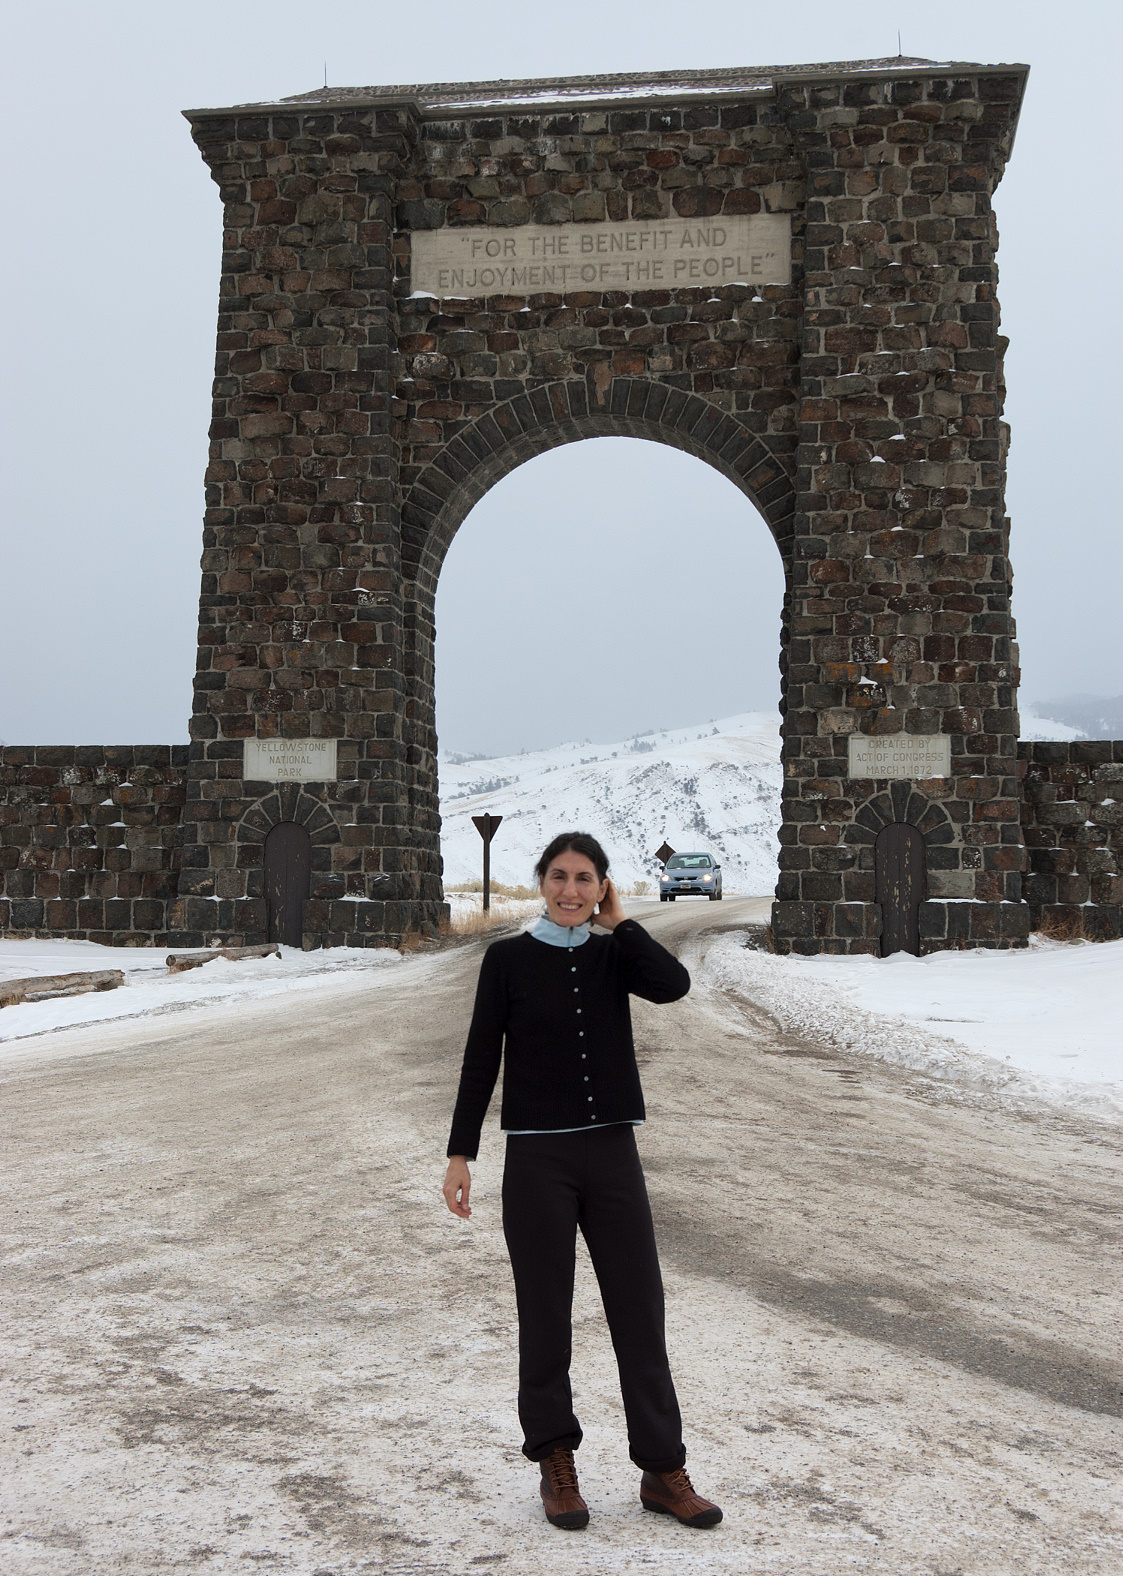
\includegraphics[width=0.32\textwidth]{mali-yellowstone-roosevelt-gate-winter.jpg}}
%\caption{My wife in front of the Roosevelt Gate that marks the northern entrance
%to Yellowstone. The road to Mammoth Hot Springs and the Lamar valley are
%open during the winter. Most of the park is snowed under.}
%\label{fig:4186X0}
%\end{floatingfigure} 

\captionsetup[figure]{labelformat=empty}
\begin{SCfigure}
\centering
\href{http://conceptcontrol.smugmug.com/Trips/USA-and-Canada/North-Western/i-cJMHzj5/A}{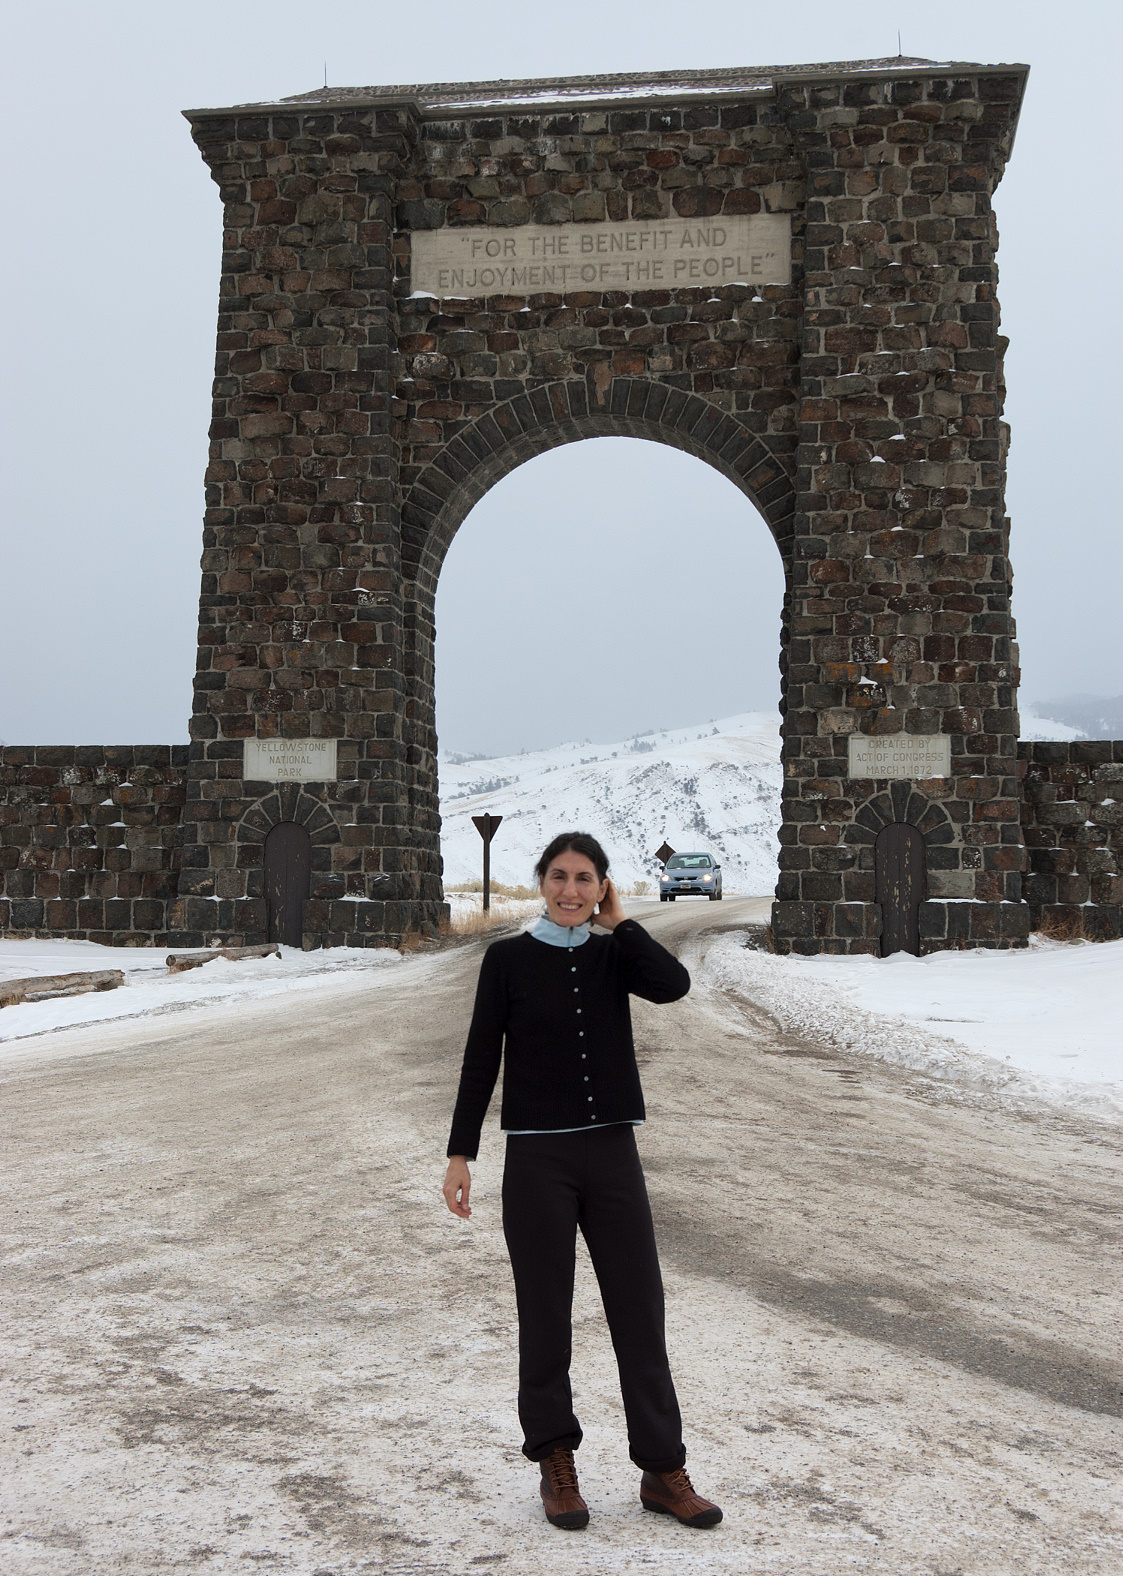
\includegraphics[width=0.32\textwidth]{mali-yellowstone-roosevelt-gate-winter.jpg}}
\caption{My wife in front of the Roosevelt Gate: the northern entrance
to Yellowstone. The road to Mammoth Hot Springs and the Lamar valley are
open during the winter but most of the park is snowed under and the roads are
closed except for snow coaches. Winter is a good time to visit the park - no crowds!}
\end{SCfigure}


I have moved so often that I am no longer from anywhere, but if asked,
one place,~\href{http://www.livingstonmontana.org/}{Livingston Montana},
has the strongest claim. Every summer, from infancy to late adolescence,
I spent long happy months with my grandparents in Livingston. If you
look at a map you'll see that Livingston is close to
\href{http://www.nps.gov/yell/index.htm}{Yellowstone National Park}. In
the late 19\textsuperscript{th} and early 20\textsuperscript{th} century
the town billed itself as the gateway to Yellowstone. In those days most
people reached the park by train and the train went through Livingston
on the way to Gardner and the northern park entrance where the famous
Teddy Roosevelt arch stands to this day.

Being close to Yellowstone we made frequent family trips to the park. I
don't know how many times I've entered Yellowstone. We'd make at least
one trip every year and some years we went two or three times. We
thought of Yellowstone as our own private national park and we were
intensely proud of the place. This hasn't changed. People that live near
the park today are as fiercely devoted to Yellowstone as my grandparents
and parents ever were.

When I was a child the park service did things differently. In the
1950's and 1960's rangers didn't chase bears into the woods so they hung
out on park roads begging food from tourists. Seeing bears closeup was
always a thrill. Of course you weren't supposed to feed bears. Signs
were everywhere reminding
\href{http://www.urbandictionary.com/define.php?term=Boobus\%20Americanus}{\emph{Boobus
americanus}} that bears were dangerous wild animals, but the largely
ignorant public ignored the warnings with predictable results. Every
year at least one moron was killed by a bear. In good years two or three
would succumb. Since most of the dead were clueless tourists locals
viewed Yellowstone bear attacks as a form of imbecile euthanasia. We
were sad when rangers had to put down offending bears. You don't see a
lot of bears in the park these days. When they show up the rangers shoo
them into the woods; it's easier to train bears than tourists.


%{[}caption id=``attachment\_4208'' align=``aligncenter''  width=``459''{]}
%\href{http://conceptcontrol.smugmug.com/People/The-Way-We-Were/i-xCDHX8z/A}{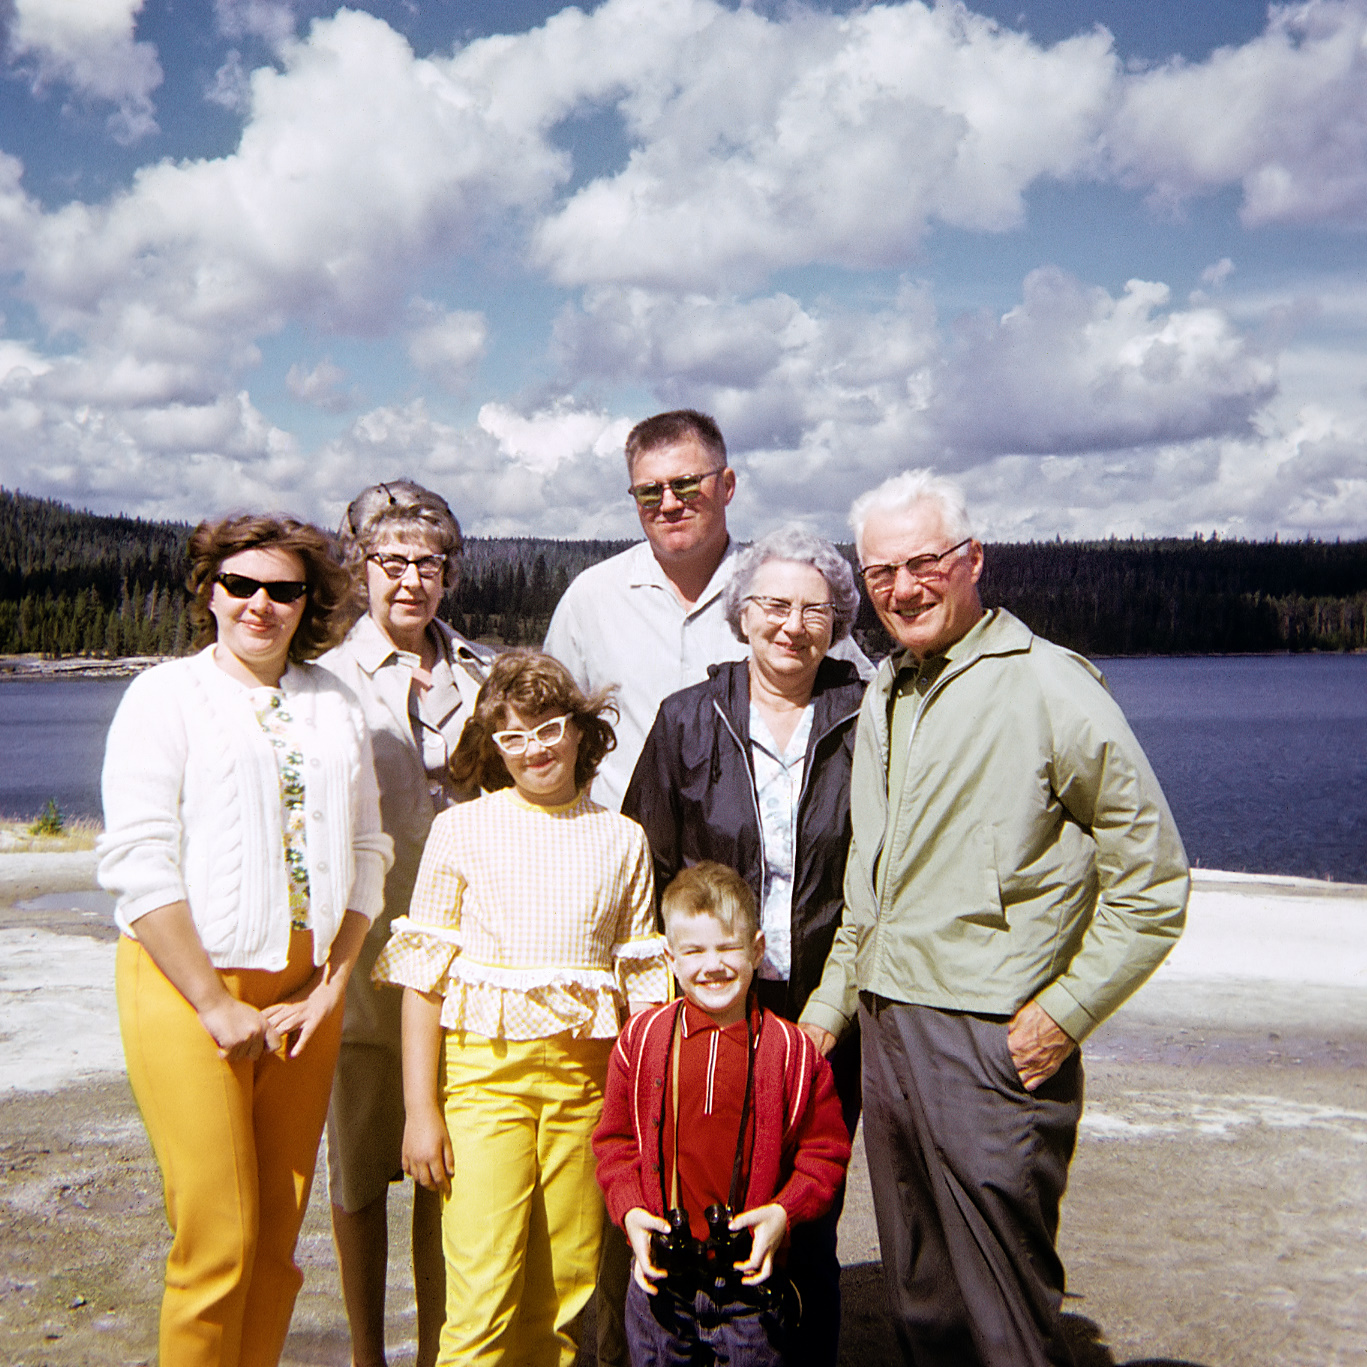
\includegraphics{bakers-and-margo-yellowstone-1967-329798671.jpg}}
%In the summer of 1967 I snapped this photo of my parents, maternal
%grandparents and siblings with an Instamatic camera. I was only a
%teenager but I was already a veteran Yellowstone visitor. We made
%frequent trips to the park and we all loved the place.
%{[}/caption{]}

%\begin{figure}[htbp]
%\centering
%\href{http://conceptcontrol.smugmug.com/People/The-Way-We-Were/i-xCDHX8z/A}{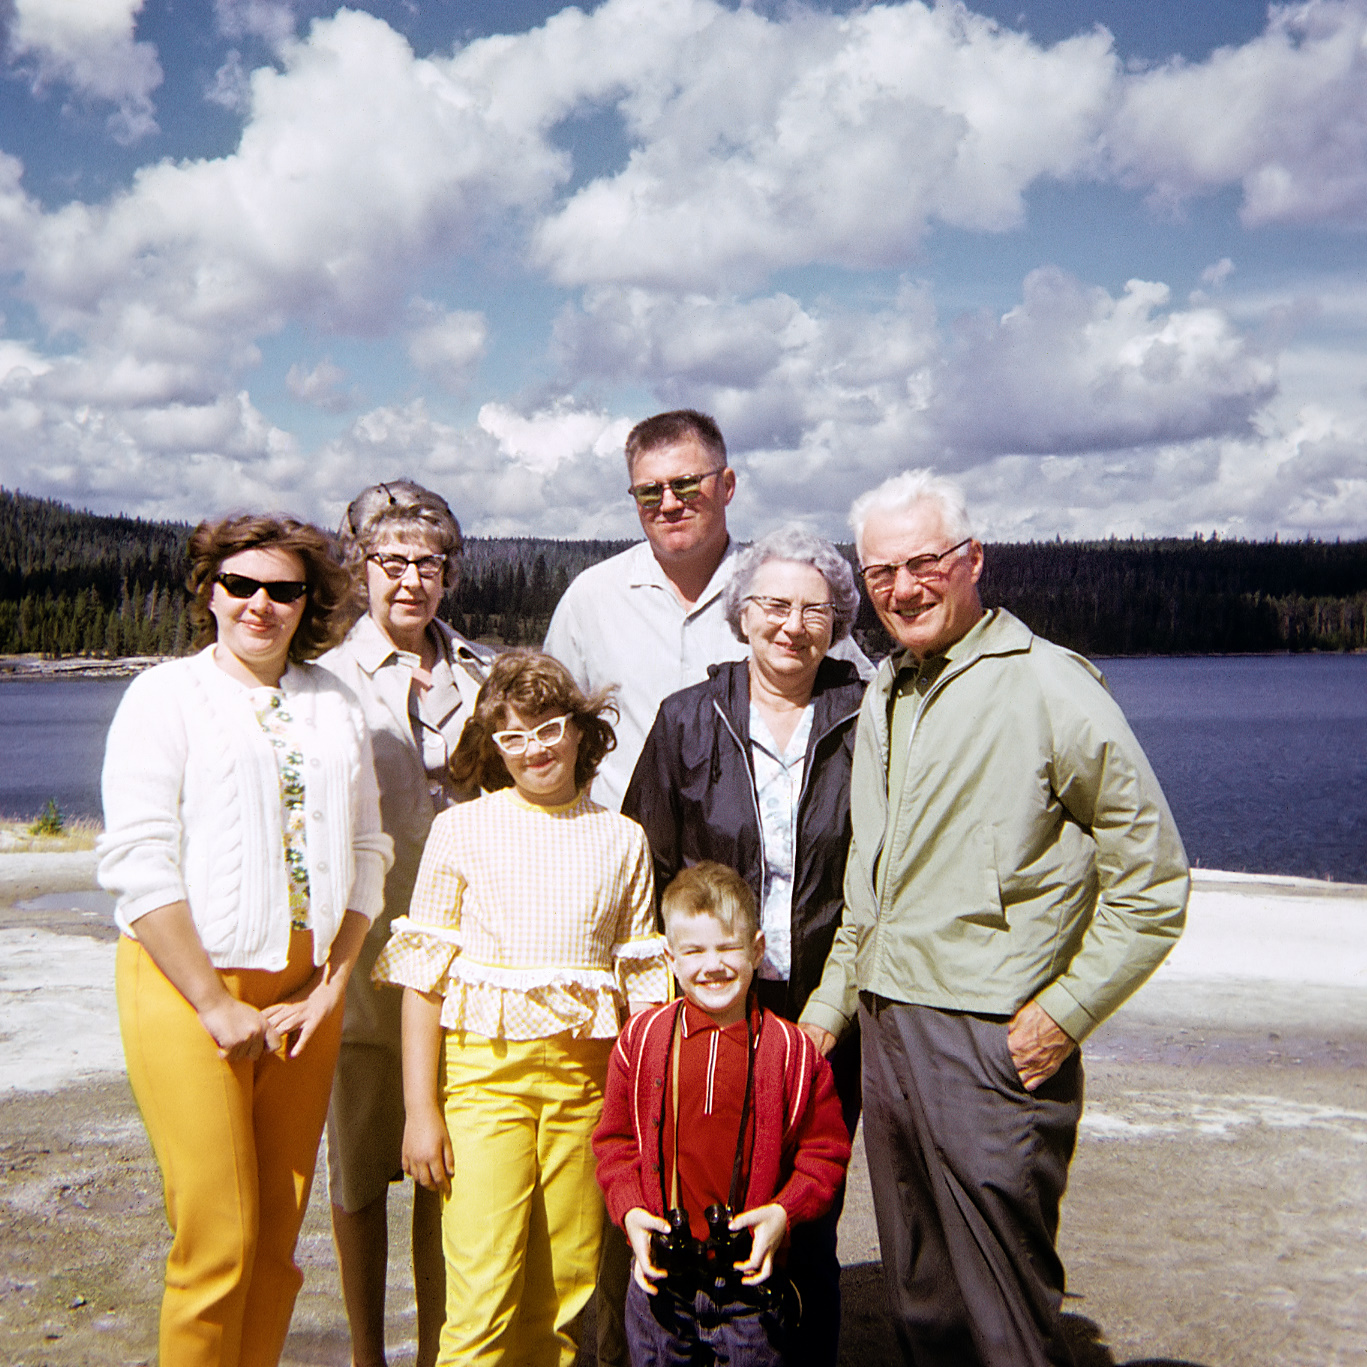
\includegraphics[width=0.45\textwidth]{bakers-and-margo-yellowstone-1967-329798671.jpg}}
%\caption{In the summer of 1967 I snapped this photo of my parents, maternal
%grandparents and siblings with an Instamatic camera. I was only a
%teenager but I was already a veteran Yellowstone visitor. We made
%frequent trips to the park and we all loved the place.}
%\label{fig:4186X1}
%\end{figure}

\captionsetup[figure]{labelformat=empty}

\begin{SCfigure}
\centering
\href{http://conceptcontrol.smugmug.com/People/The-Way-We-Were/i-xCDHX8z/A}{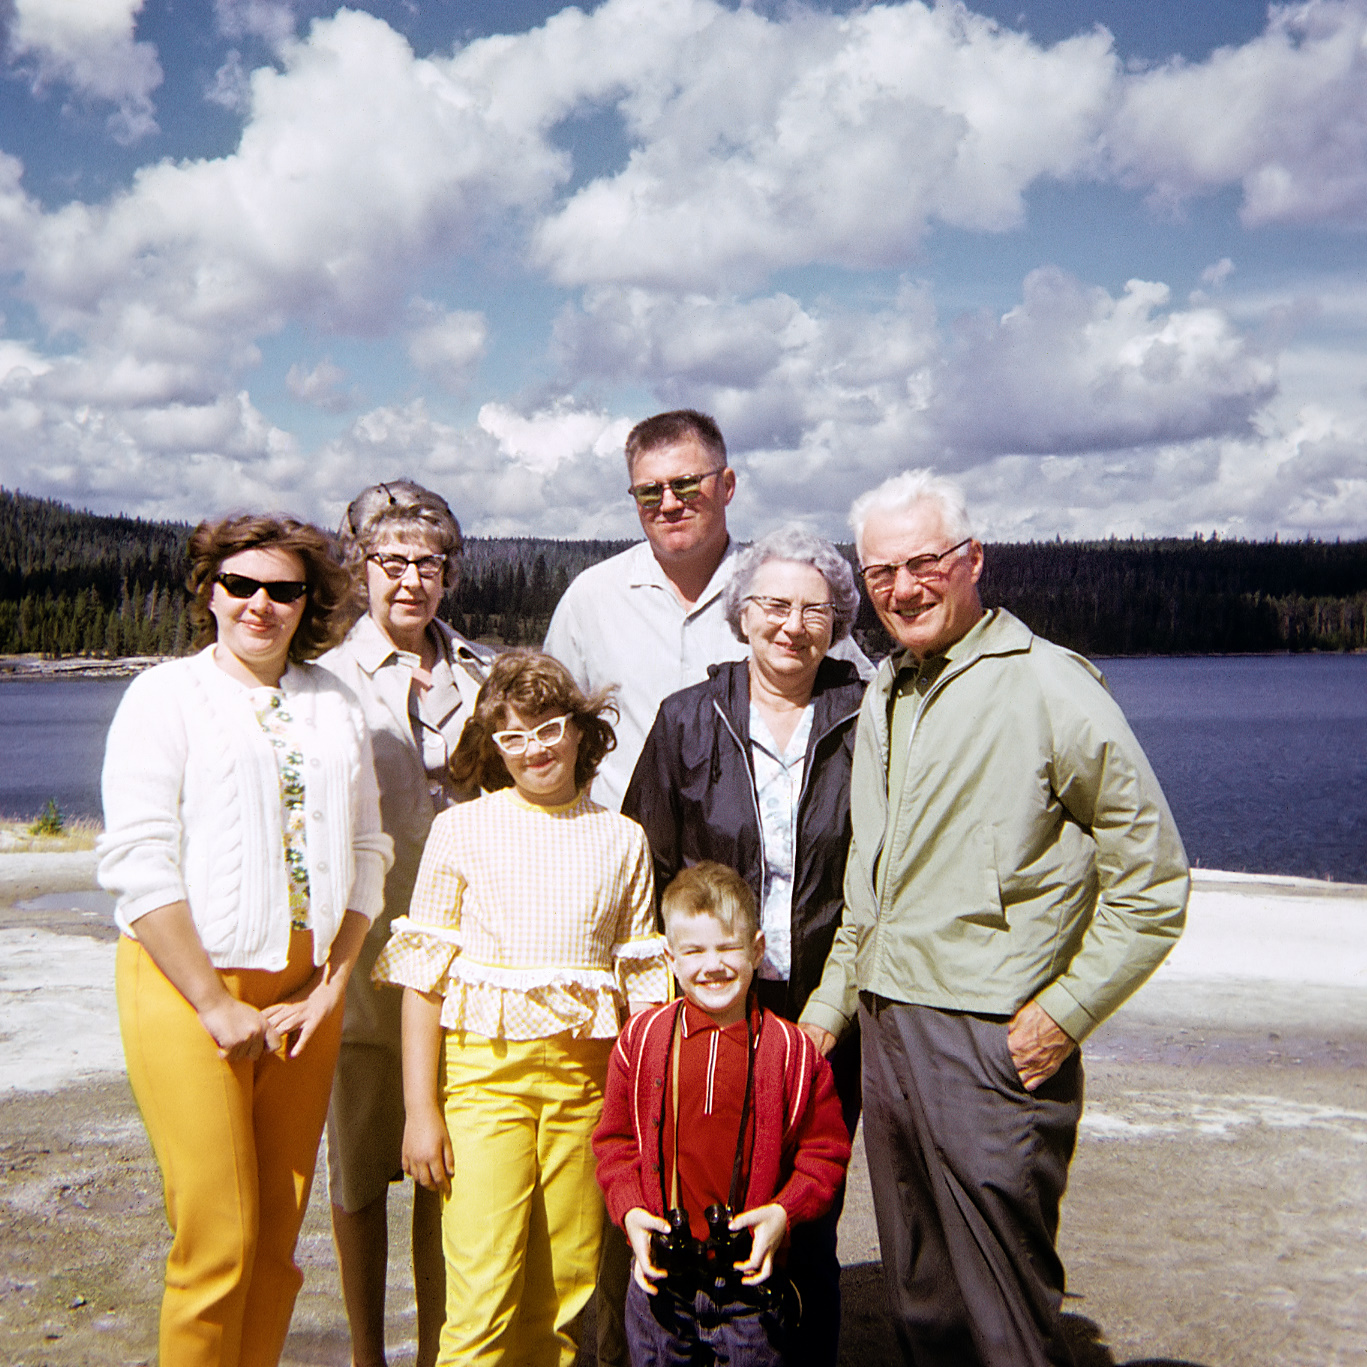
\includegraphics[width=0.40\textwidth]{bakers-and-margo-yellowstone-1967-329798671.jpg}}
\caption{In the summer of 1967 I snapped this photo of my parents, maternal
grandparents and siblings with an Instamatic camera. I was only a
teenager but I was already a veteran Yellowstone visitor. We made
frequent trips to the park and we all loved the place.}
\label{fig:4186X1}
\end{SCfigure}

After bears geysers were the next biggest thrill. Yellowstone is
world-famous for its geysers. Some estimate that half of the worlds
active geysers are bubbling away atop Yellowstone's massive caldera. The
immense size and power of the Yellowstone super-volcano was not fully
understood in those days but you could see the park was a special,
almost magical, place with your own eyes. One geyser,
\href{http://www.nps.gov/yell/planyourvisit/noldfaith.htm}{Old
Faithful}, is emblematic of Yellowstone and most of our park trips
included a stop at it.

Old Faithful is not the most spectacular large geyser in the park but
it's the most dependable. By some rare geological quirk Old Faithful has
been venting at regular intervals ever since it was named in
1870.\footnote{
Nobody knows who first discovered Old Faithful. It was known to Native
Americans long before it was named ``Old Faithful.''
} The interval changes a bit from
time to time. The
\href{http://en.wikipedia.org/wiki/1959\_Yellowstone\_earthquake}{Madison
earthquake} tweaked the frequency and times vary more than many believe,
but if you go to Old Faithful and invest a few hours the geyser will not
disappoint. The most dramatic eruptions occur during the winter when
super-heated geyser steam blasts into freezing mountain plateau air. Old
Faithful in the winter is pure bucket list material. I've watched Old
Faithful shoot off dozens of times. I've seen Old Faithful with my
parents, my siblings, my grandparents, my children, my nieces, in-laws
and some good friends. My experience is not unique. If you've seen Old
Faithful I'm betting it was with someone special.

There's more to Yellowstone than bears and geysers. It harbors the
largest high altitude lake in North America. It is home to a variety of
North American plants and animals. It has one of the most spectacular
river canyons and waterfalls anywhere and it shelters, in scalding
geyser waters, rare ancient
\href{http://en.wikipedia.org/wiki/Extremophile}{extremophiles} that are
among the oldest life forms on Earth. The park doesn't need me to sell
it. It's one of the world's very special places.


%{[}caption id=``attachment\_4211'' align=``aligncenter''  width=``406''{]}
%\href{http://conceptcontrol.smugmug.com/People/My-Kids/i-wMwM8mG/A}{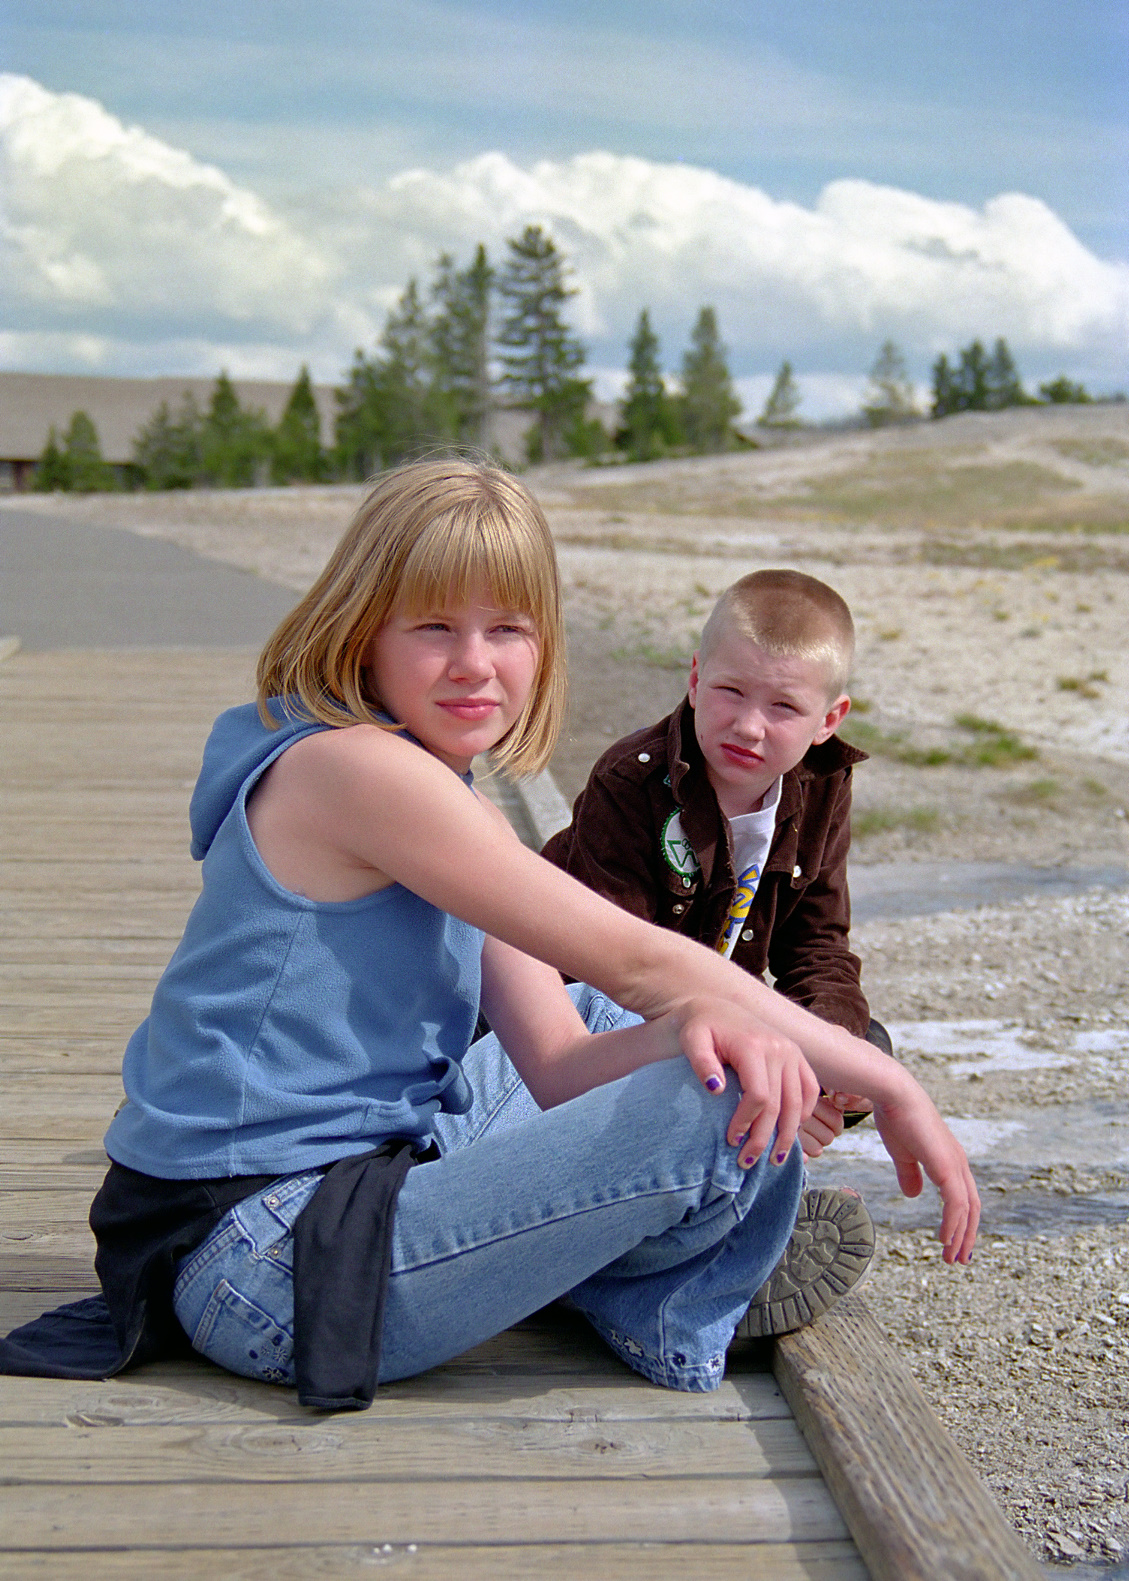
\includegraphics{helen-jacob-old-faithful-2000.jpg}}
%My kids waiting for Old Faithful to erupt in the summer of 2000.
%Watching Old Faithful is like a family reunion for me. I've seen it
%shoot off with most of the special people in my life and even when I was
%by myself I was always thinking how others would love this particular
%eruption.
%{[}/caption{]}

\begin{SCfigure}
\centering
\href{http://conceptcontrol.smugmug.com/People/My-Kids/i-wMwM8mG/A}{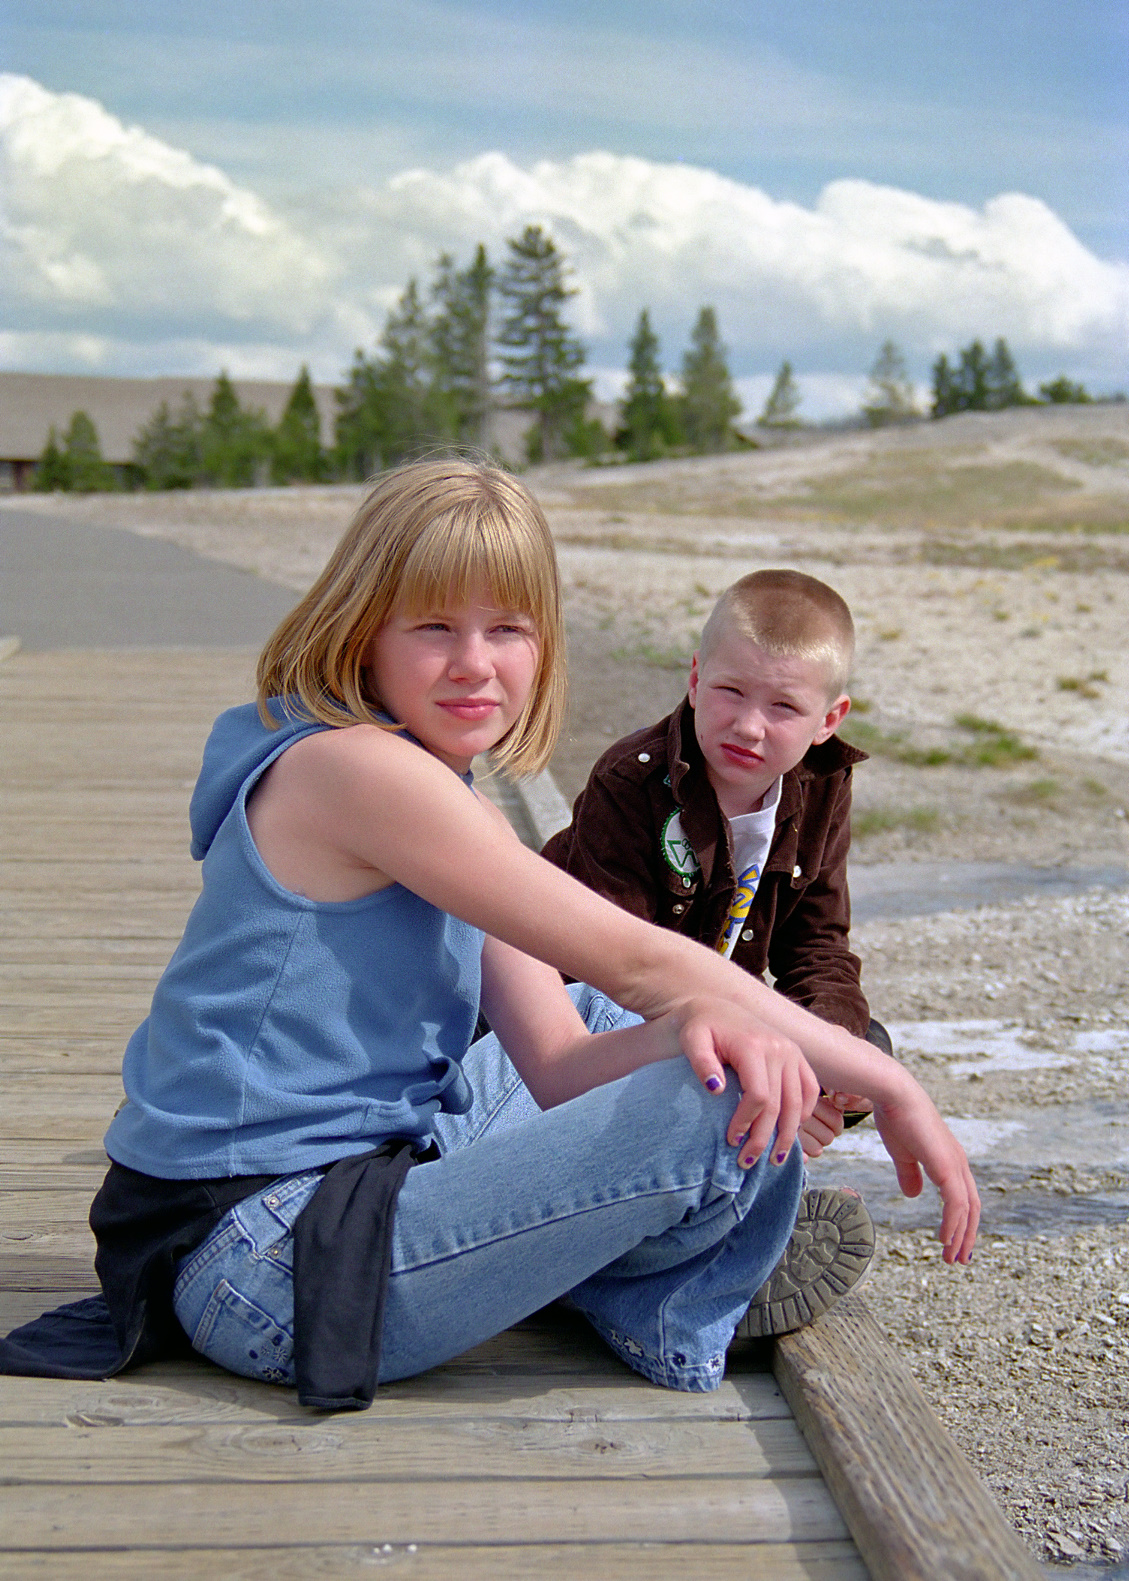
\includegraphics[width=0.40\textwidth]{helen-jacob-old-faithful-2000.jpg}}
\caption{My kids waiting for Old Faithful to erupt in the summer of 2000.
Watching Old Faithful is like a family reunion for me. I've seen it
shoot off with most of the special people in my life and even when I was
by myself I was always thinking how others would love this particular
eruption.}
\label{fig:4186X2}
\end{SCfigure}


As I entered my teenage years we moved to Iran where I spent a year
before moving to Lebanon for school. During this time I saw large chunks
of the Middle East, Egypt, Turkey, most of Western Europe and England.
We returned to Canada. From Canada I moved to Ghana, then Denmark, then
Barbados, then western Canada, then eastern Canada, then back to the US.
I've seen dozens of national parks in many countries and many are
spectacular. With so much to compare it against I started thinking of
Yellowstone as, ``a been there, done that'', ``nothing to see here'',
``not worth the hassle,'' bore! Doesn't everyone have a boring old
Yellowstone in their backyard? I was blasé~about Yellowstone for years
until two notable events and advances in geology made me reassess my
feelings about the park.

Remember the great Yellowstone
\href{http://en.wikipedia.org/wiki/Yellowstone\_fires\_of\_1988}{forest
fires of 1988}. Dramatic images of vast fires filled newscasts for
weeks. The park service endured abuse from all quarters for letting the
fires rage. Fire has always been important for North American evergreen
forests. Years of fire suppression in the US and Canada slowly produced
dense tinderbox forests that blaze when set alight. The great
Yellowstone fires of 1988 punctuated this point. We now understand that
fire is necessary for the long-term health of forests, but explaining
this to outfitters, tour operators and other businesses that depend on
moving tourists in and out of parks remains a hard sell. A few years
after the great 1988 fires I visited the park with my young children. I
was expecting a burned out wasteland but I was surprised by verdant
undergrowth and the largest fattest elk herds I had ever seen. Between
the black timbers lush ferns and other plants burst forth by the
billions. It was a good time for ungulates. I know it pisses people off
when experts are right but the experts were right about forest fires.
Fortunately the braying nitwits soon had something even more
controversial to whine about.

The most famous animal in the park these days was absent during my
youth. I am talking about wolves. Wolves had been exterminated in
Yellowstone for the usual fallacious bullshit reasons in the early
20\textsuperscript{th} century. When people started seriously
entertaining the idea of reintroducing wolves to the park every
brain-dead rancher in the west decided to go on TV and show the world
that westerners are every bit as ignorant as Yellowstone bear-food
tourists. I remember one particularly eye-rolling twit going on about
how kids waiting for school buses at lonely winter ranch gates would
fall prey to bloodthirsty wolves. It didn't matter that there have been
very few \emph{authenticated} wolf attacks on people or that there were
good ecological reasons for reintroducing wolves. Ranchers the world
over subscribe to what I call rancher ecology. \emph{If it's not a cow
or a rancher shoot it!} I've endured this sentiment in the US, Canada,
Brazil and Ghana. Grow up people; you're embarrassing us! If you're
really this stupid having bloodthirsty wolves pick off your idiot spawn
would help us maintain our species IQ.

The park service ignored the loons and brought the wolves back. What
happened, just the biggest and most successful species reintroduction in
national park history? Watching wolves reestablish themselves has made
it crystal clear how important top predators are to functional
ecosystems. Before the wolves came back the elk and deer, like welfare
recipients, had gotten stupid and lazy. Their biggest problem was
avoiding traffic. The wolves changed all that. Now if they're not on
their hooves they're probably going to get eaten. The presence of wolves
has had many unexpected benefits. The elk no longer clear out the
underbrush near streams; this has led to a profusion of wild flowers and
other plants that were rarely seen before wolves. The denser plant
growth has provided habit for insects that feed birds. The slower moving
waters are more suitable for native fish and beavers. The park is in
better shape than it has been at any time in my life and we can credit
the work of \emph{Canis lupus} for a lot of it.


%{[}caption id=``attachment\_4215'' align=``aligncenter''  width=``1610''{]}
%\href{http://conceptcontrol.smugmug.com/Trips/USA-and-Canada/North-Western/i-j7WcGTK/A}{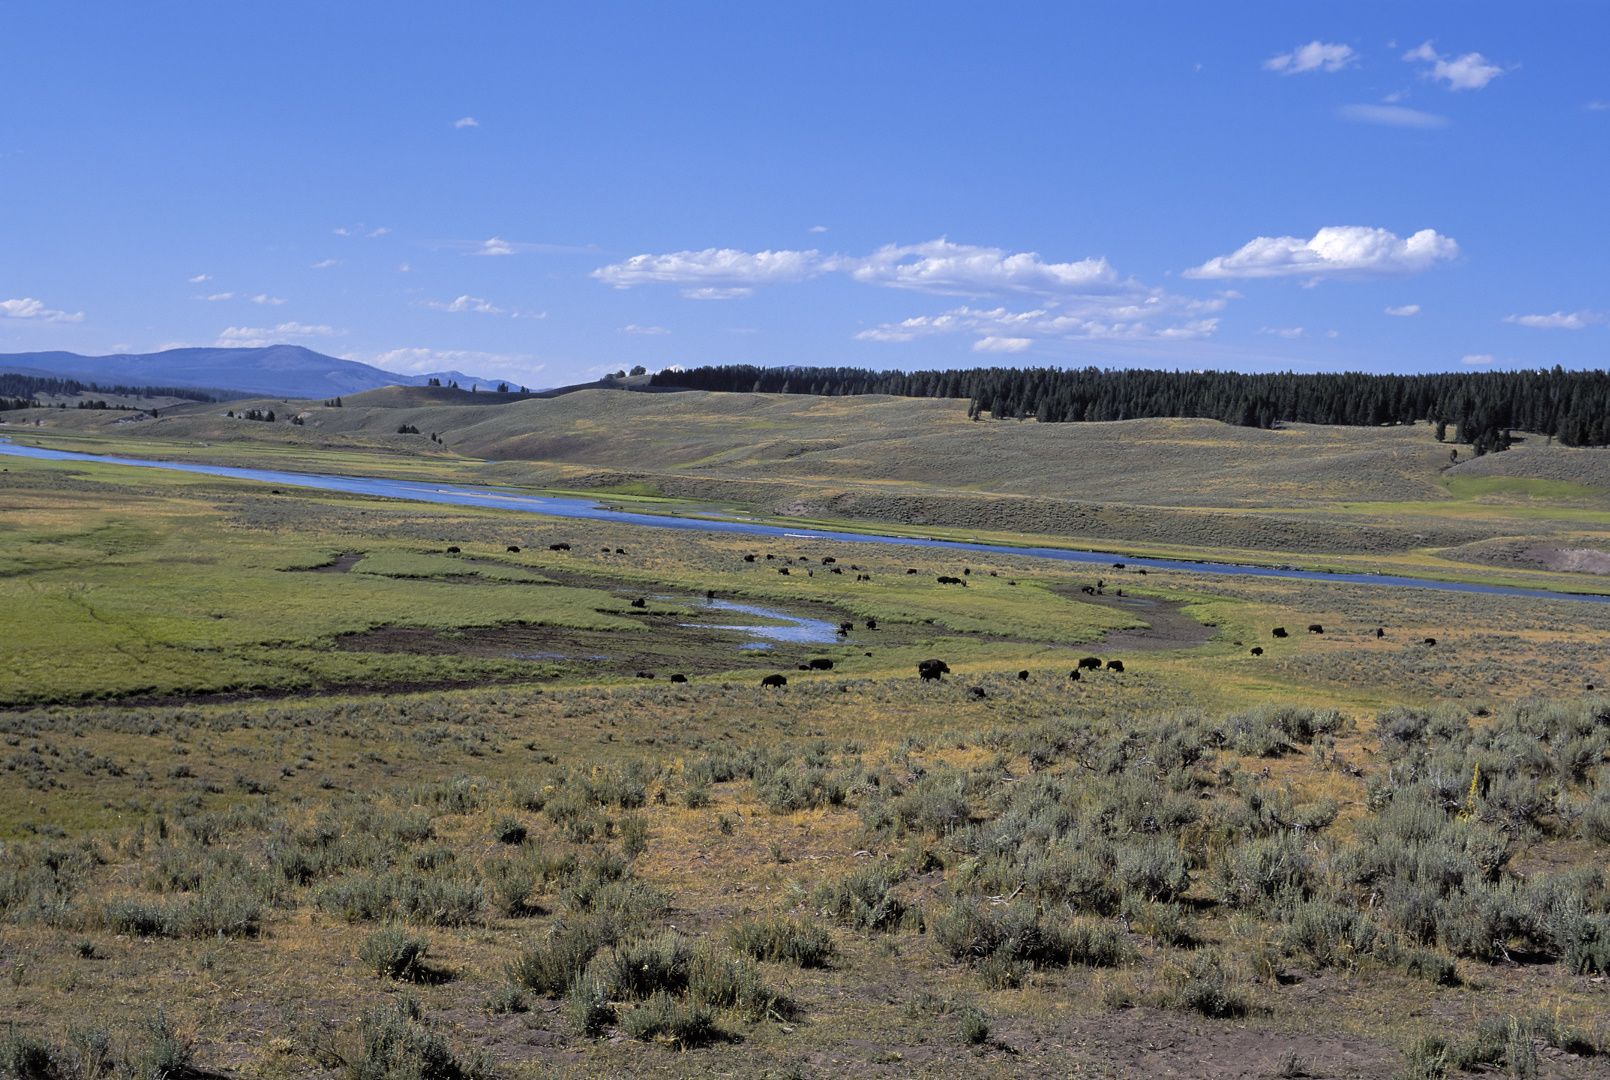
\includegraphics{yellowstone-bison-plain-4441253.jpg}}
%Most of Yellowstone is a high elevation plateau. It's great habitat for
%deer, elk, bears and now wolves. There are mountains in the park but
%they are not as impressive as the Tetons to the south or the Absaroka
%range to the north.
%{[}/caption{]}

\begin{SCfigure}
\centering
\href{http://conceptcontrol.smugmug.com/Trips/USA-and-Canada/North-Western/i-j7WcGTK/A}{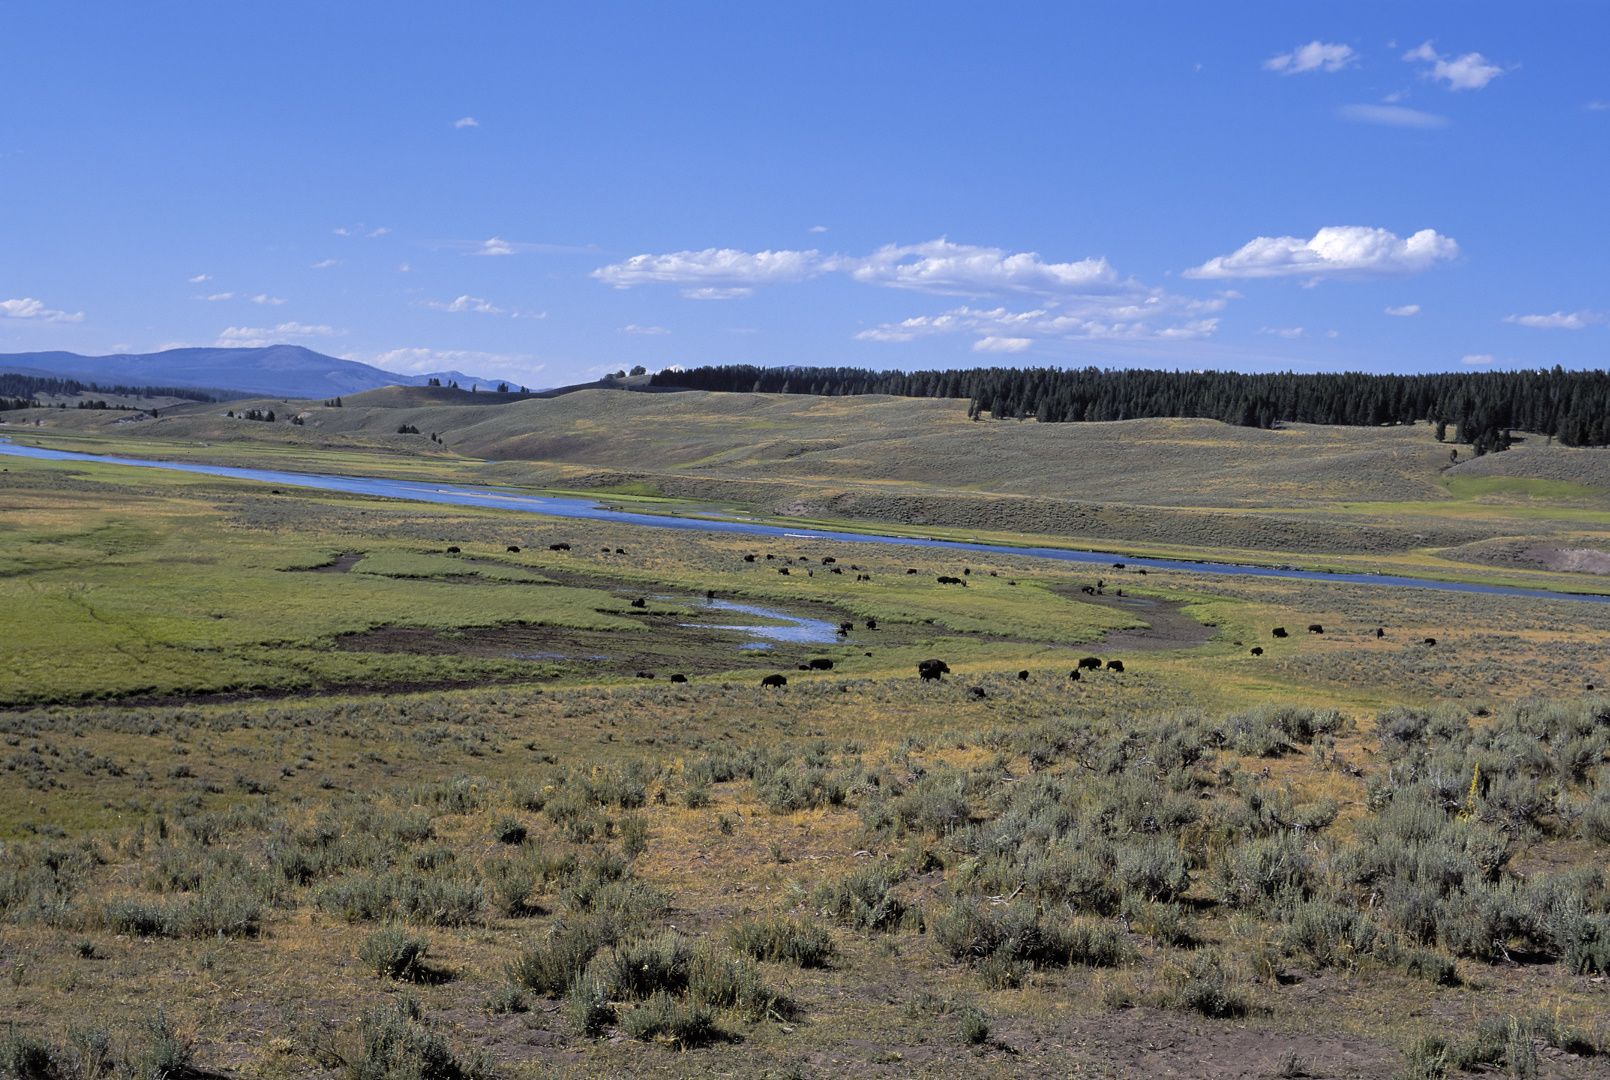
\includegraphics[width=0.50\textwidth]{yellowstone-bison-plain-4441253.jpg}}
\caption{Most of Yellowstone is a high elevation plateau. It's great habitat for
deer, elk, bears and now wolves. There are mountains in the park but
they are not as impressive as the Tetons to the south or the Absaroka
range to the north.}
\label{fig:4186X3}
\end{SCfigure}


And, despite the western whining, the biggest beneficiaries of wolf
reintroduction have been, you guessed it: \emph{Homo sapiens.} Lots of
people are making money on Yellowstone wolves. Every winter thousands of
people make their way into the Lamar valley to watch and hear wolves.
People come from far and wide and occasionally the wolves put on a
riveting show for them. Yes they occasionally stray from the park and
there have been livestock losses. Whenever a sheep of calf gets eaten
the rancher press covers it like a mini 9/11 terrorist attack. In some
cases the attacks \emph{occur in the park}. It's not widely known that
domestic animals graze national forests and parks. Hey, if your cow is
eating state subsidized grass stop whining about occasional losses to
wildlife. You're damn lucky the stupid public tolerates grazing on
public lands. In pure economic terms wolf introduction has been a rare
government money-maker. Perhaps if
\href{http://www.urbandictionary.com/define.php?term=congress}{\emph{Congress
assholus}} were reintroduced to their natural habit, \emph{prison},
similar benefits would ensue.

Wolf reintroduction put Yellowstone back in the news but advances in
geophysics and geology vaulted the park's status to global icon. There
aren't very many
\href{http://wiki.answers.com/Q/How\_many\_super\_volcanoes\_are\_there\_all\_together\_in\_the\_world}{super
volcanoes in the world} and there are even fewer active super-volcanoes.
This is probably a good thing. Too many of these puppies blowing off
would seriously depress the market and no amount of quantitative easing
would excavate your baked ass from cubic kilometers of volcanic ash.
Geologists have been aware of Yellowstone's violent volcanic past for
decades but it wasn't until the age of high precision GPS monitoring and
satellite radar that the alarming dynamism of the park made headlines.
We're not used to landscapes ``breathing'' but something like that is
going on in the Yellowstone caldera. The entire plateau goes up and down
in amazingly short times. It takes a lot of energy to move a few hundred
square kilometers of rock in a matter of years. Yellowstone ground
movements have been monitored since the 1920's and they are so marked
that even the public notices. Now that we better understand
\href{http://ngm.nationalgeographic.com/2009/08/yellowstone/yellowstone-interactive}{the
monster that lurks under the park} everyone expects it to wake one day
and blow the joint sky-high. Maybe we'll get lucky and see it blow in
our lifetime. The last time the Yellowstone super-volcano erupted
\emph{Homo erectus} walked the Earth. They we're on the other side of
the world but super-volcanoes make themselves felt at great distances.
I'm willing to bet that evidence of large Yellowstone eruptions will
eventually be detected in ancient African or Asian hominid fossils.
Yellowstone's super-volcano gives the park real sex appeal. Let's face
it, chicks dig bad boys, and bad boys that can waste entire countries
are volcanically hot!


%{[}caption id=``attachment\_4204'' align=``aligncenter''  width=``1607''{]}
%\href{http://conceptcontrol.smugmug.com/Trips/USA-and-Canada/North-Western/i-6R2qMdw/A}{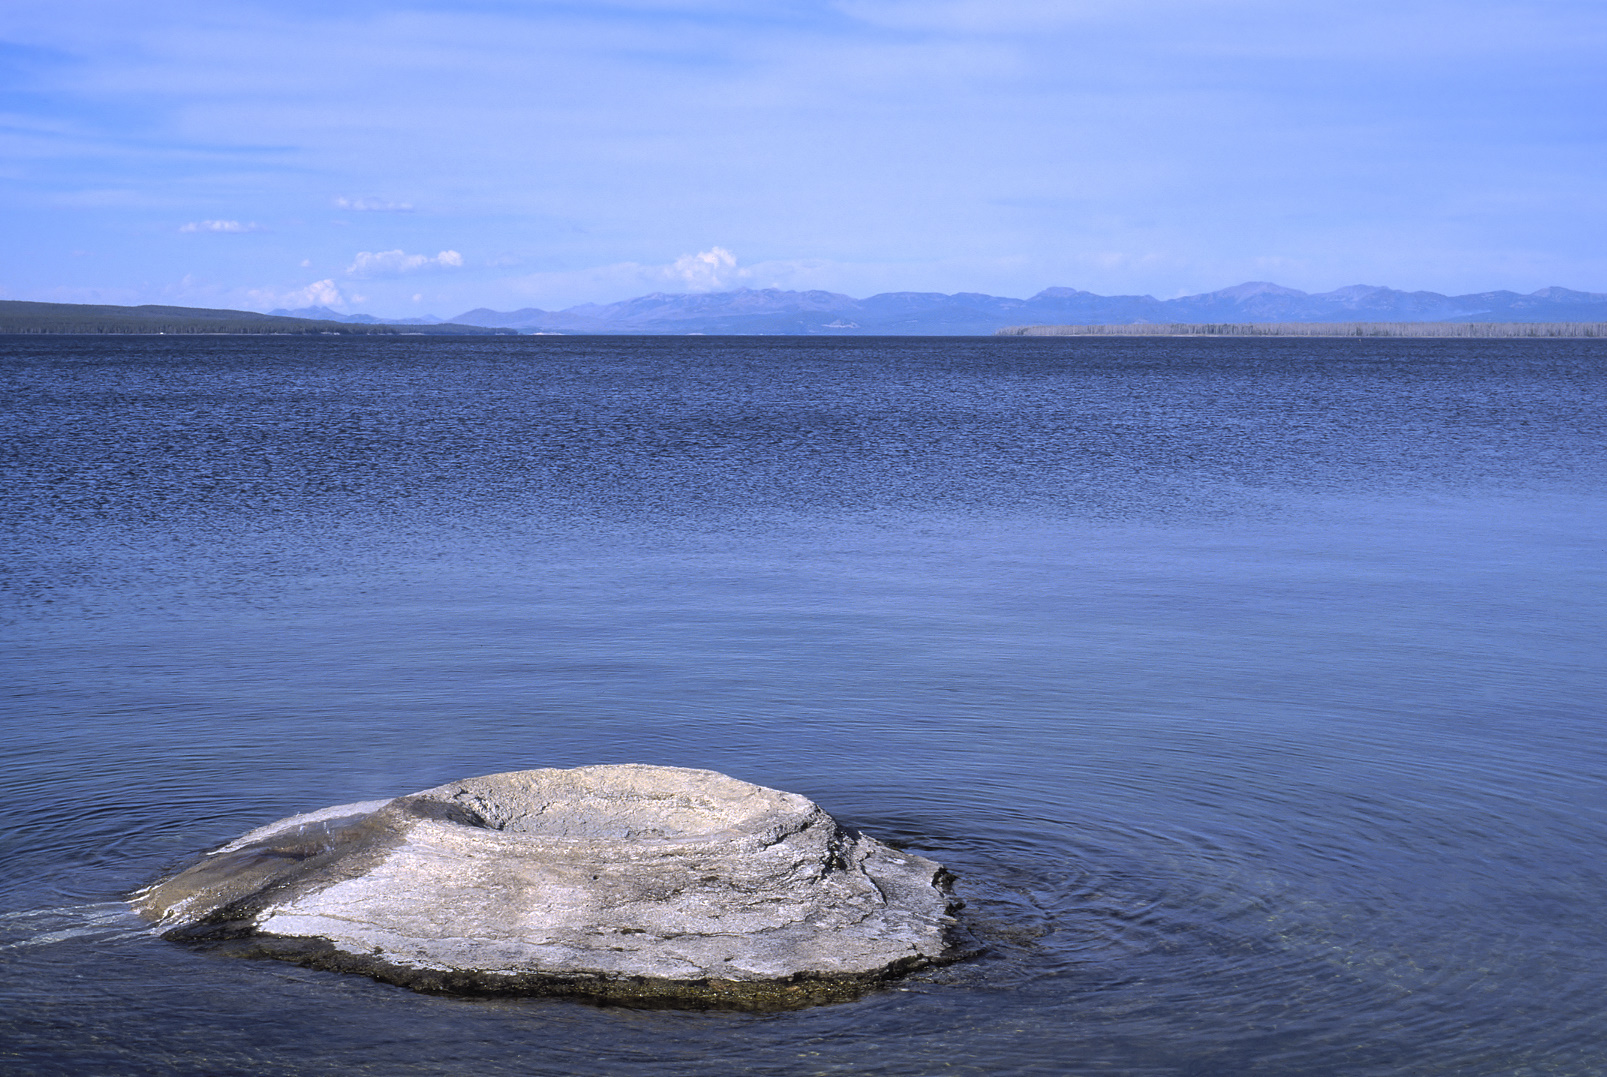
\includegraphics{geyser-yellowstone-lake-2242391.jpg}}
%Yellowstone Lake from West Thumb. Yellowstone Lake is large and deep and
%most of it lies within the Yellowstone caldera which covers an area
%three times larger than the lake. Imagine this entire landscape
%erupting. They're not called super-volcanoes for nothing!
%{[}/caption{]}

\begin{SCfigure}
\centering
\centering
\href{http://conceptcontrol.smugmug.com/Trips/USA-and-Canada/North-Western/i-6R2qMdw/A}{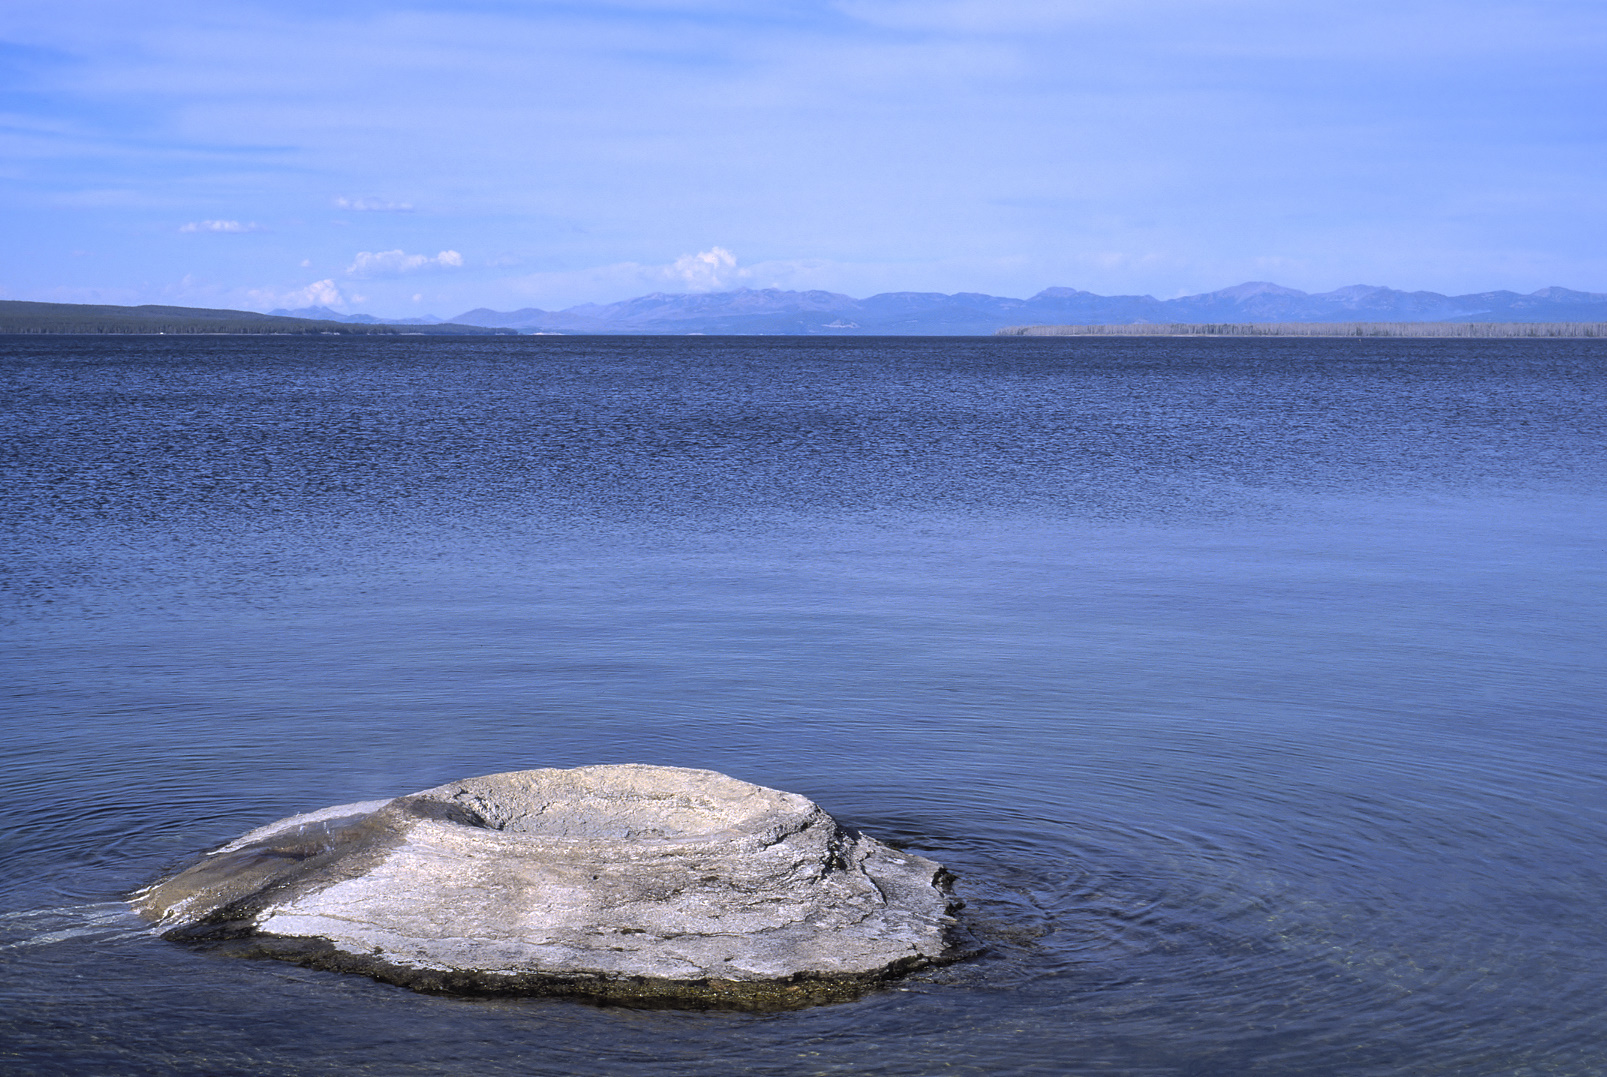
\includegraphics[width=0.50\textwidth]{geyser-yellowstone-lake-2242391.jpg}}
\caption{Yellowstone Lake from West Thumb. Yellowstone Lake is large and deep and
most of it lies within the Yellowstone caldera which covers an area
three times larger than the lake. Imagine this entire landscape
erupting. They're not called super-volcanoes for nothing!}
\label{fig:4186X4}
\end{SCfigure}


Yellowstone's enduring importance has nothing to do with landscapes,
geysers, bears or volcanoes. Its major contribution is the \emph{idea of
a national park.} In 1872 the US Congress took time out from their usual
whoring and profiteering, work they assiduously pursue to this day, and
accidentally did something worthwhile; they created the world's first
national park: Yellowstone. Despite modern whitewashing this wasn't an
act of a farsighted and wise people. Yellowstone was too far away, too
high for agriculture, had no known mineral deposits and wasn't even in a
state at the time. How the hell can you deliver pork to nonexistent
districts? Congress couldn't see how to pillage and profit from
Yellowstone so they gave in to a small but determined movement that
wanted a park. The congress of 1872 was probably less corrupt and venal
than our modern degenerates but they weren't freaking saints and it
annoys the hell out of me that partisan revisionists are constantly
citing Yellowstone as a wonder of big government. Yellowstone was a
product of the corrupt and incompetent
Grant\footnote{
Unlike the current occupant of the White House Grant did something
that mattered before he was elected president.
} administration for Christ's sake.
The same dolts that brought you Custer's last stand.

Judging the motivations of the long dead is pure hubris but evaluating
the results of their actions is how we learn from history. By any
standard Yellowstone was a glorious result. The congress of 1872 set a
precedent that spread worldwide.
\href{http://www.pbs.org/nationalparks/}{Ken Burns} argues that national
parks are the single best idea the US government has ever had and I
agree. \emph{I shudder to think what Yellowstone would be like if it
wasn't a national park.} It would probably be the biggest hive of luxury
spas and posturing celebrity scum on the planet. Imagine Aspen, Cannes,
Bath, Monte Carlo, Dubai and Hollywood all whored up with natural
boiling mud and geyser waters. Instead of being proud of Yellowstone I
would be advocating nuking the place. The nukes wouldn't damage the
super-volcano but they would cauterize the celebrity infestation. Thank
the \href{http://www.venganza.org/}{all squiggling FSM} that this
nightmare was aborted in 1872. National parks have aborted many such
nightmares all around the globe.

In my ideal world parks would cover at least a third of Earth's lands
and oceans. We're not there yet, but when we are, people will still look
at Yellowstone, the world's first national park, and my personal
favorite, as one of the very best.

%\begin{center}\rule{3in}{0.4pt}\end{center}
%
%\begin{enumerate}
%\item
%  Nobody knows who first discovered Old Faithful. It was known to Native
%  Americans long before it was named ``Old
%  Faithful.''\hyperref[fnref1]{↩}
%\item
%  Unlike the current occupant of the White House Grant did something
%  that mattered before he was elected president.\hyperref[fnref2]{↩}
%\end{enumerate}

%\captionsetup[floatingfigure]{labelformat=empty}
%\begin{figure}[htbp]
%\begin{floatingfigure}[l]{0.25\textwidth}
%\centering
%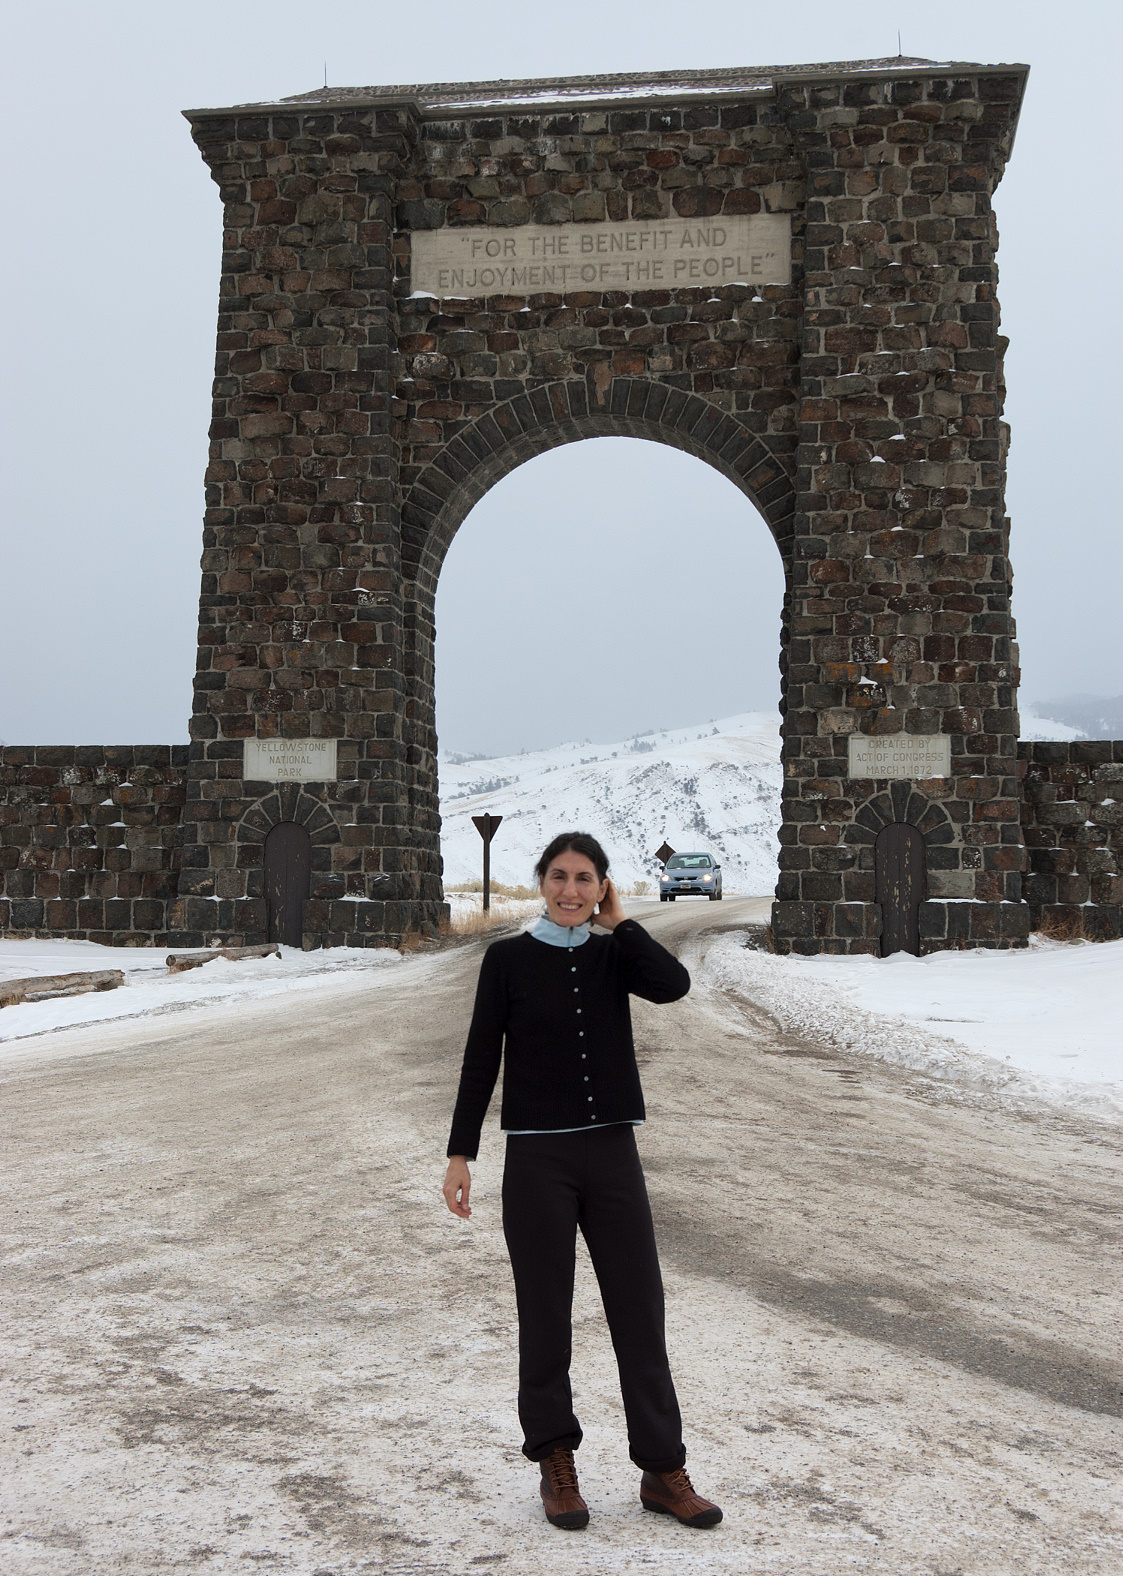
\includegraphics[width=0.23\textwidth]{mali-yellowstone-roosevelt-gate-winter.jpg}
%\caption{~~~IMCAPTION~~~}
%\label{fig:4186X0}
%\end{floatingfigure}
%\end{figure}

%\captionsetup[floatingfigure]{labelformat=empty}
%\begin{figure}[htbp]
%\begin{floatingfigure}[l]{0.25\textwidth}
%\centering
%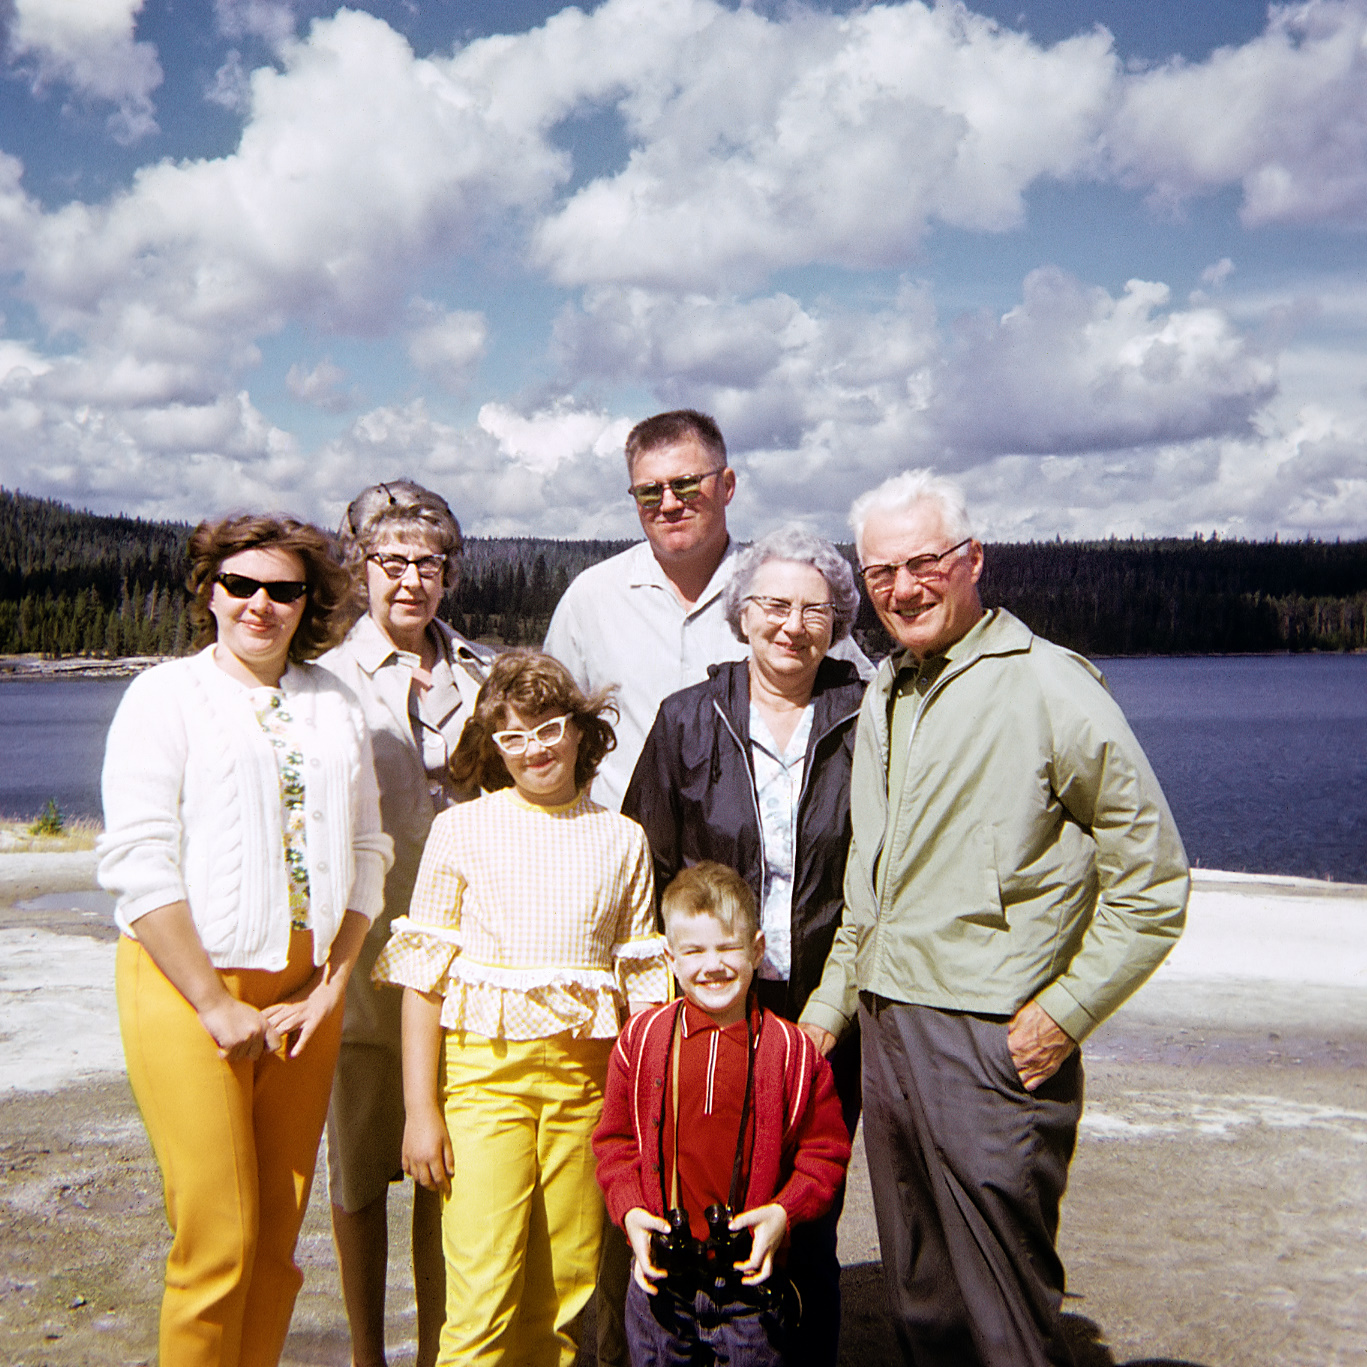
\includegraphics[width=0.23\textwidth]{bakers-and-margo-yellowstone-1967-329798671.jpg}
%\caption{~~~IMCAPTION~~~}
%\label{fig:4186X1}
%\end{floatingfigure}
%\end{figure}

%\captionsetup[floatingfigure]{labelformat=empty}
%\begin{figure}[htbp]
%\begin{floatingfigure}[l]{0.25\textwidth}
%\centering
%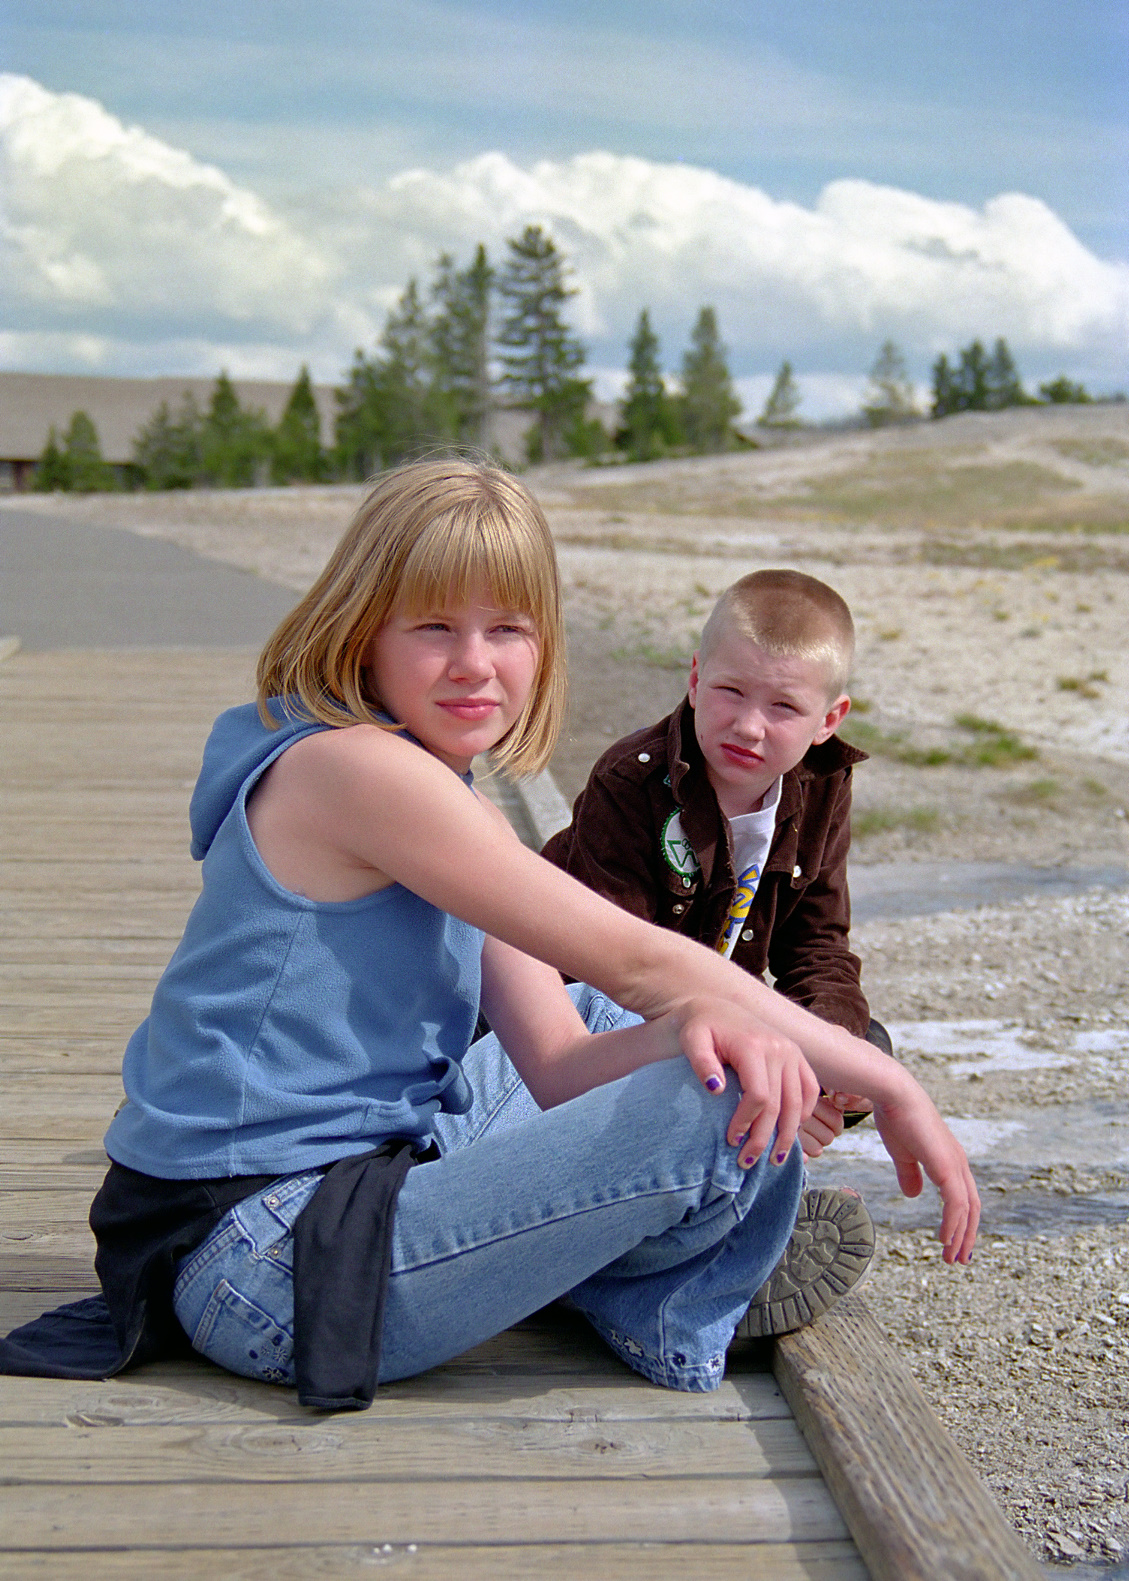
\includegraphics[width=0.23\textwidth]{helen-jacob-old-faithful-2000.jpg}
%\caption{~~~IMCAPTION~~~}
%\label{fig:4186X2}
%\end{floatingfigure}
%\end{figure}

%\captionsetup[floatingfigure]{labelformat=empty}
%\begin{figure}[htbp]
%\begin{floatingfigure}[l]{0.25\textwidth}
%\centering
%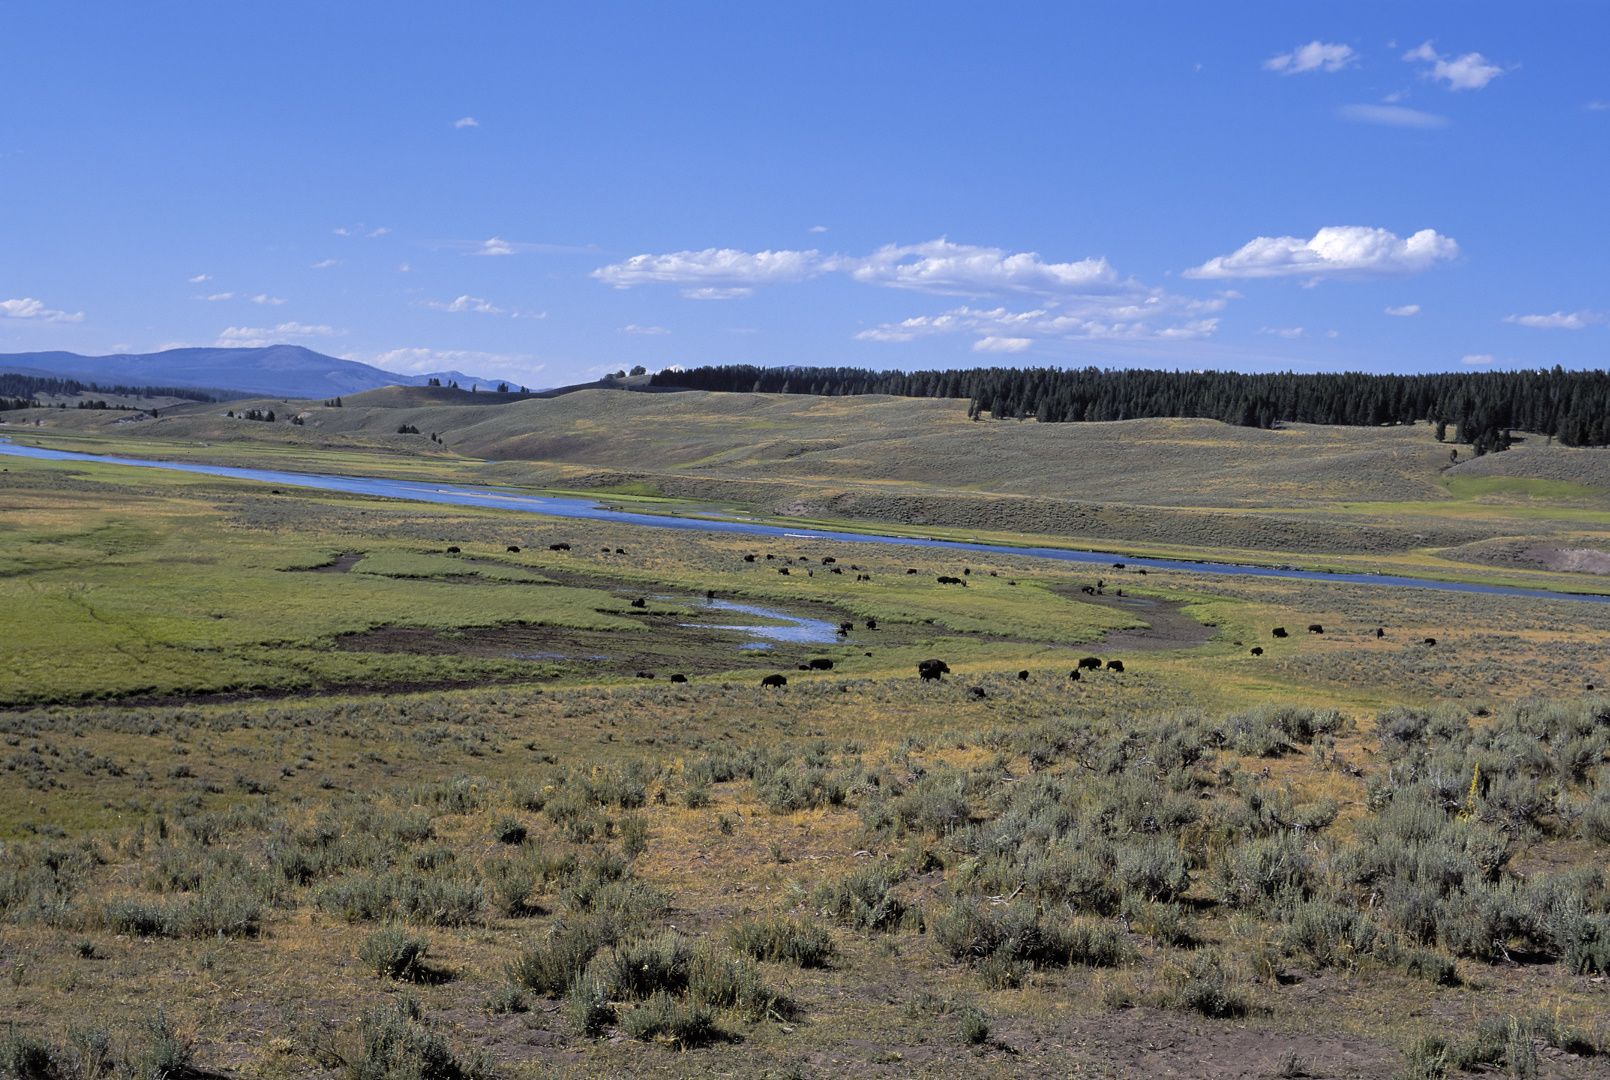
\includegraphics[width=0.23\textwidth]{yellowstone-bison-plain-4441253.jpg}
%\caption{~~~IMCAPTION~~~}
%\label{fig:4186X3}
%\end{floatingfigure}
%\end{figure}

%\captionsetup[floatingfigure]{labelformat=empty}
%\begin{figure}[htbp]
%\begin{floatingfigure}[l]{0.25\textwidth}
%\centering
%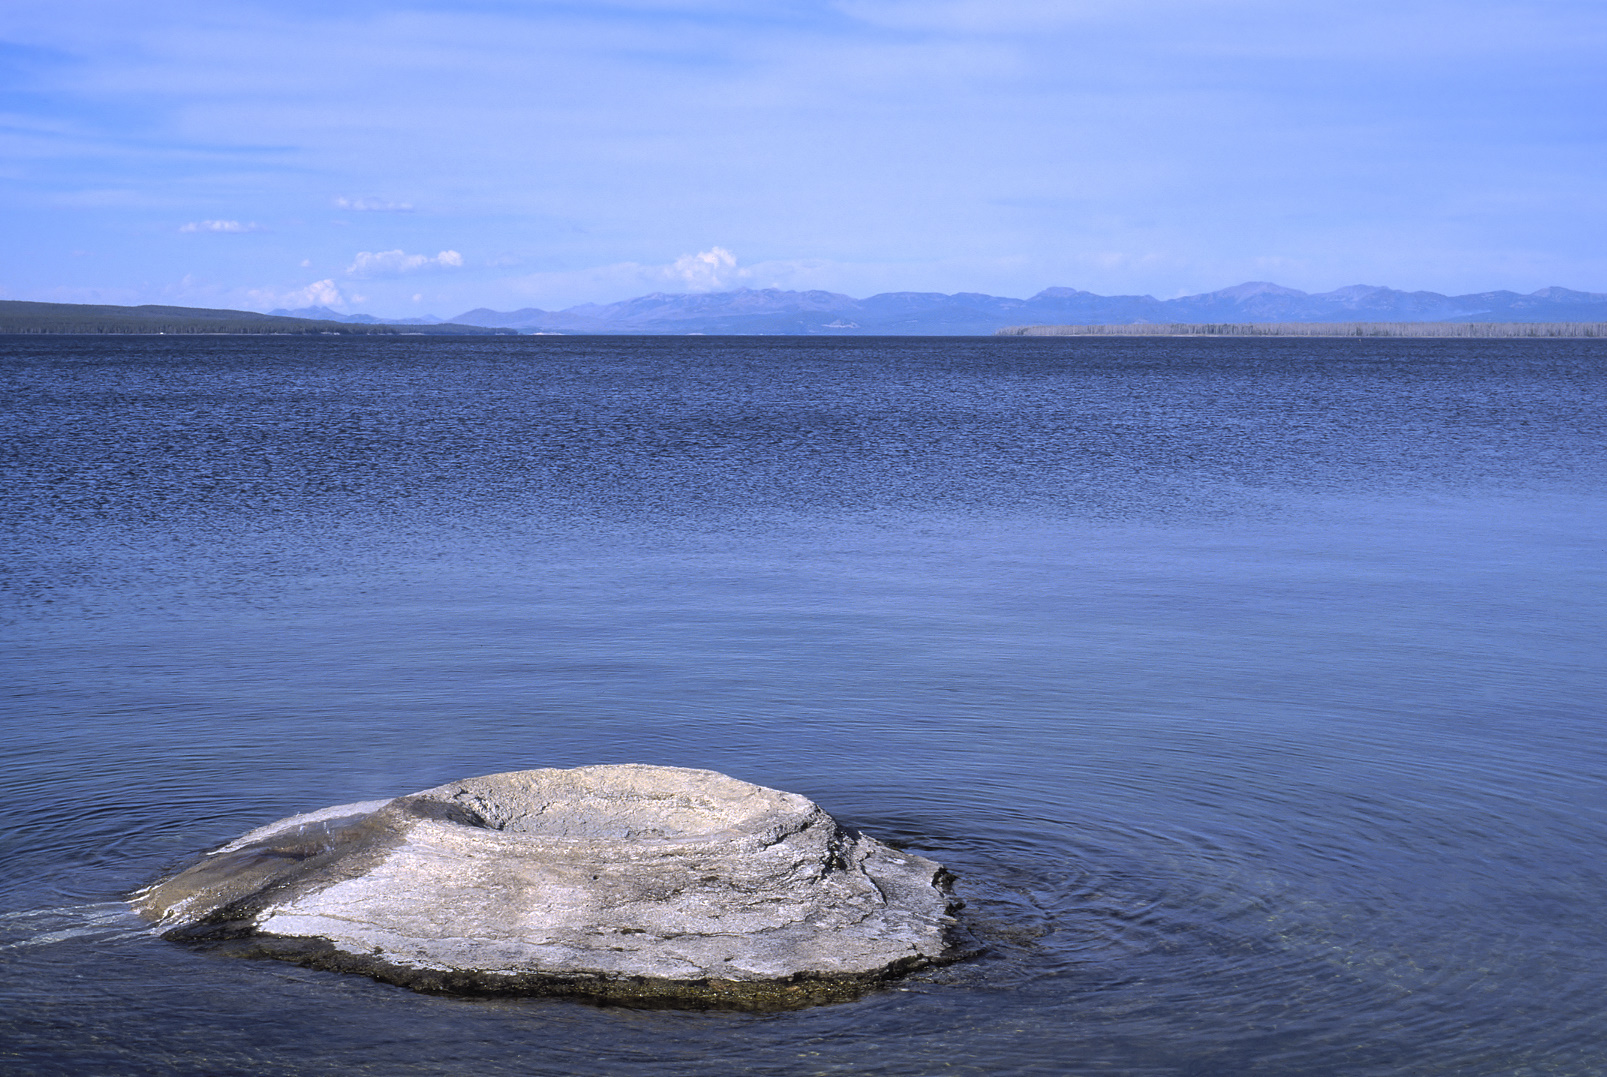
\includegraphics[width=0.23\textwidth]{geyser-yellowstone-lake-2242391.jpg}
%\caption{~~~IMCAPTION~~~}
%\label{fig:4186X4}
%\end{floatingfigure}
%\end{figure}



%\end{document}